\documentclass[12pt]{extarticle}
%Some packages I commonly use.
\usepackage[english]{babel}
\usepackage{graphicx}
\usepackage{framed}
\usepackage[normalem]{ulem}
\usepackage{amsmath}
\usepackage{amsthm}
\usepackage{amssymb}
\usepackage{amsfonts}
\usepackage{enumerate}
\usepackage[utf8]{inputenc}
\usepackage[top=1 in,bottom=1in, left=1 in, right=1 in]{geometry}
\usepackage{xeCJK}
\usepackage{physics}
\usepackage{hyperref}
\usepackage{multicol}

% \usepackage{tabularx,booktabs}


% \graphicspath{ {./images/} }
\numberwithin{equation}{section}
\numberwithin{figure}{section}
\numberwithin{table}{section}


%A bunch of definitions that make my life easier
\newcommand{\matlab}{{\sc Matlab} }
\newcommand{\cvec}[1]{{\mathbf #1}}
\newcommand{\rvec}[1]{\vec{\mathbf #1}}
\newcommand{\ihat}{\hat{\textbf{\i}}}
\newcommand{\jhat}{\hat{\textbf{\j}}}
\newcommand{\khat}{\hat{\textbf{k}}}
\newcommand{\minor}{{\rm minor}}
% \newcommand{\trace}{{\rm trace}}
\newcommand{\spn}{{\rm Span}}
\newcommand{\rem}{{\rm rem}}
\newcommand{\ran}{{\rm range}}
\newcommand{\range}{{\rm range}}
\newcommand{\mdiv}{{\rm div}}
\newcommand{\proj}{{\rm proj}}
\newcommand{\R}{\mathbb{R}}
\newcommand{\N}{\mathbb{N}}
\newcommand{\Q}{\mathbb{Q}}
\newcommand{\Z}{\mathbb{Z}}
\newcommand{\<}{\langle}
\renewcommand{\>}{\rangle}
\renewcommand{\emptyset}{\varnothing}
\newcommand{\attn}[1]{\textbf{#1}}
\theoremstyle{definition}
\newtheorem{theorem}{Theorem}
\newtheorem{corollary}{Corollary}
\newtheorem*{definition}{Definition}
\newtheorem*{example}{Example}
\newtheorem*{note}{Note}
\newtheorem{exercise}{Exercise}
\newcommand{\bproof}{\bigskip {\bf Proof. }}
\newcommand{\eproof}{\hfill\qedsymbol}
\newcommand{\Disp}{\displaystyle}
\newcommand{\qe}{\hfill\(\bigtriangledown\)}


\newcommand{\SubItem}[1]{
    {\setlength\itemindent{15pt} \item[-] #1}
}
\newcommand{\Lap}{\boldsymbol{\bigtriangledown}}
\newcommand{\chiOne}{{{\chi^{(1)}}_x}^x}
\newcommand{\chiThree}{{{\chi^{(3)}}_x}^{xxx}}

\setlength{\columnseprule}{1 pt}


\title{Nonlinear Fiber Optics\cite{agrawal_nonlinear_2007} Summary}
\author{Maodong Gao}
\date{\today}

\begin{document}

\maketitle
\tableofcontents
\newpage


\section{Introduction}
    \subsection{Historical prospective}
    
        \begin{itemize}
            \item 1960, fibres lossy $\geq$ 1000dB/km. 1970 20dB/km.
            \item 1979, loss level 0.2dB/km in 1.55um. Limited by Rayleigh Scattering.
            \item 1972, Raman and Brillouin scattering process are studied using optical fibers.
            \item Stimulated other nonlinear phenomena,including optically induced birefringence, parametric 4-wave mixing, self-phase modulation
            \item 1973, soliton like pulses are suggested. 1980 observed. 6fs pulse observed in 1987.
            \item 1990s, Erbium-doped fiber amplifier, wavelength near 1550nm.
            \item 2000s, stimulated Raman scattering(so called Raman amplification), four-wave mixing(so called Fiber-optic parametric amplifiers) are two new types of amplifiers. Do not require doped atoms and spectral region not limited.
            \item Amplifiers fueled optical solitons. New types of solitons such as dispersion-managed solitons and dissipative solitons.
            \item (Chapter 11) 1978, fibre gratings. 1996, New types of fibers, such as photonic crystal fibres, crystal fibers,  holey fibers and micro-structure fibers.
            \item (Chapter 12) New types of fibers has new dispersive (GVD, group velocity dispersion) and nonlinear (relativity small core size enhance nonlinear effects) properties.
            \item (Chapter 13) Supercontinuum generation. optical spectrum of incident light broadens by a factor of $\geq$100 over a short length of fiber.
        \end{itemize}
    
    \subsection{Fiber Characteristics}
        \begin{itemize}
            \item step-index fibers, see \autoref{fig1.1}.
            \item Two parameters characterize optical fiber: relative core-cladding index difference; V parameter.
            \item core-cladding index difference:
                \begin{equation}
                    \Delta = \frac{n_1 - n_c}{n_1}
                    \label{core-cladding index difference}
                \end{equation}
            \item V parameter: this parameter determines number of modes supported by this fiber at a certain wavelength $\lambda$. Fiber supports single mode of a certain $\lambda$ if $V < 2.405$.
                \begin{equation}
                    V = k_0 a \sqrt{n_1^2 - n_c^2}
                    \label{V parameter}
                \end{equation}
            where a is core radius, $k_0 = \frac{2\pi}{\lambda}$
        \end{itemize}
    
        \begin{figure}[htbp]
            \centering
            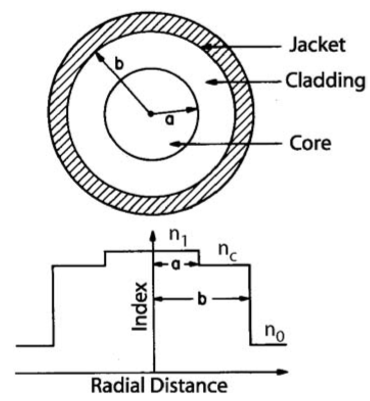
\includegraphics[width=0.4\textwidth]{images/fig1.1.PNG}
            \caption{Schematic illustration of the cross section and the refractive-index profile of a stepindex fiber.}
            \label{fig1.1}
        \end{figure}
        
        \subsubsection{Material and Fabrication}
            \begin{figure}[htbp]
                \centering
                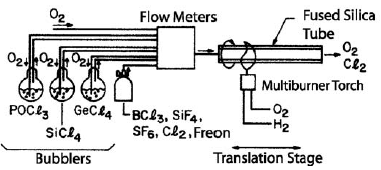
\includegraphics[width=0.6\textwidth]{images/fig1.2.PNG}
                \caption{Schematic diagram of the MCVD process commonly used for fiber fabrication.}
                \label{fig1.2}
            \end{figure}
            
            \begin{itemize}
                \item Dopants increase refractive index: $GeO_2, P_2O_5$.
                \item Dopants decrease refractive index: $boron, fluorine$
                \item Dopants to core for amplification: $ErCl_3, Nd_2O_3$
                \item MCVD(modified chemical vapor deposition) fiber fabrication process.
            \end{itemize}
            
        \subsubsection{Fiber Losses}
            Losses are characterized by attenuation constant $\alpha$:
                \begin{equation}
                    P_T = P_0 \exp{(-\alpha L)}.
                    \label{attenuation constant}
                \end{equation}
            Another unit for $\alpha$ is dB/km, which are related by:
                \begin{equation}
                    \alpha_{dB} = -\frac{10}{L}\log{(\frac{P_T}{P_0})} = 4.343\alpha
                \end{equation}
            A high loss up to 10dB/km corresponds to attenutation constant of \\
            $\alpha \approx 2 km^{-1} = 2\times 10^{-5}cm^{-1} $,
            which is already very low compared to most other materials.
            
            
            \begin{figure}[htbp]
                \centering
                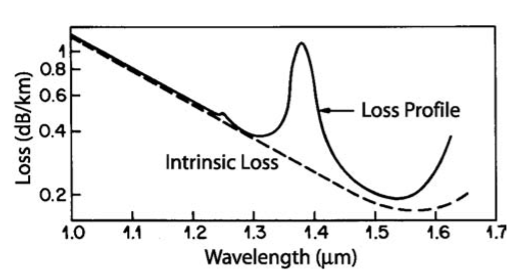
\includegraphics[width=0.6\textwidth]{images/fig1.3.PNG}
                \caption{Measured loss spectrum of a single-mode silica fiber. Dashed curve shows the contribution resulting from Rayleigh scattering.}
                \label{fig1.3}
            \end{figure}
            
            Two main fiber loss channels: Rayleigh scattering; Material absorption.
            \begin{itemize}
                \item Raleigh scattering, arises from density fluctuation frozen into fused silica.Local fluctuations in refractive index, scatter lights into all directions.
                    \begin{equation}
                        \alpha_R = \frac{C_R}{\lambda^4}
                    \end{equation}
                    Raleigh scattering strength decreases rapidly as wavelength increases. $C_R$ depends on constituents of fiber core, typically around $0.7-0.9 dB/(km \mu m^4)$. As $\alpha_R$ around $0.12-0.15 dB/km$ near $\lambda = 1.55 \mu m$.
                \item Material absorption: Silica glass electronic resonance (ultraviolet region), vibrational resonance (far-infrared region beyond $2 \mu m$). Absorbs little light from $0.5 \mu m$ to $2 \mu m$.
                \item Impurity absorption: most important impurity is OH ion. Its fundamental vibrational absorption peak is at $\approx 2.73 \mu m$. The peak in \autoref{fig1.3} is the second overtone of OH ions.
            \end{itemize}
            
        \subsubsection{Chromatic Dispersion}
            \begin{itemize}
                \item Chromatic dispersion basically is reflective index over optical frequency $n(\omega)$.
                \item $n(\omega)$ relation with material resonance is well approximated by Sellmeier equation:
                    \begin{equation}
                        n^2(\omega) = 1 + \sum_{j=1}^m \frac{B_j \omega_j^2}{\omega_j^2-\omega^2},
                        \label{sellmeier equation}
                    \end{equation}
                    where $\omega_j$ are material resonances frequencies, $B_j$ is the strength of $j$th resonance. $\omega_j$ contributes more as it is nearer to frequcney of interest $\omega$.
                \item For bulk-fused silica, the fitting of Sellmeier equation to $m = 3$ has the parameters in \autoref{bulk-fused silica Sellmeier equation fitting}. This is useful when doing COMSOL simulation. The $n(\omega)$ results are shown in \autoref{fig1.4}.
                    \begin{table}[htbp]
                    \centering
                        \begin{tabular}{|c|c|c|c|}
                        \hline
                        \multicolumn{4}{|c|}{Fitting coefficients in \autoref{sellmeier equation} for bulk-fused silica up to order m=3} \\
                        \hline
                        $j$ in \autoref{sellmeier equation} & 1       & 2           & 3           \\ \hline
                        $B_j$                          & 0.6961663   & 0.4079426   & 0.8974794   \\ \hline
                        $\lambda_j / nm$               & 68.4043     & 116.2414    & 9896.161    \\ \hline
                        $\omega_j =2\pi c/\lambda_j$   & 2.7537E+16  & 1.62047E+16 & 1.90342E+14 \\ \hline
                        Freq /THz                      & 43.82655155 & 25.79050648 & 0.302938137 \\ \hline
                        \end{tabular}
                    \caption{bulk-fused silica Sellmeier \autoref{sellmeier equation} fitting}
                    \label{bulk-fused silica Sellmeier equation fitting}
                    \end{table}
                \item Dispersion induce short optical pulse broadening.
                \item Dispersion and non-linearity are different behavior components. In nonlinear regime, these two may behave qualitatively different.
                
                \item Group index $n_g$: Define $n_g = \frac{v_g}{c}$. From mode-propagation constant $\beta$ view, Taylor expands $\beta(\omega)$ about the center pulse freq $\omega_0$, 
                    \begin{equation}
                        \beta(\omega) = n(\omega)\frac{\omega}{c}=\beta_0 + \beta_1(\omega-\omega_0)+\frac{1}{2}\beta_2(\omega-\omega_0)^2,
                        \label{propagation constant expansion}
                    \end{equation}
                    where
                    \begin{equation}
                        \beta_m = (\dv[m]{\beta}{\omega})_{\omega=\omega_0}.
                        \label{betam definition}
                    \end{equation}
                    (You can treat \autoref{propagation constant expansion} as precise currently, which we will discuss later precisely at \autoref{beta omega expands around omega 0}.)\\
                    And $n_g$ are related to $\beta_1$ by:
                    \begin{equation}
                        \beta_1 = \frac{1}{v_g} = \frac{n_g}{c} = \frac{1}{c}(n+\omega \dv{n}{\omega}).
                        \label{group velocity and group index}
                    \end{equation}
                
                \item Group velocity dispersion (GVD): characterized by $\dv{n_g}{\omega}$, and this is related to $\beta_2$ by:
                    \begin{equation}
                        \beta_2 = \dv{\beta_1}{\omega} = \frac{1}{c}\dv{n_g}{\omega} = \frac{1}{c}(2\dv{n}{\omega} +\dv[2]{n}{\omega}).
                        \label{beta2 definition}
                    \end{equation}
                    In standard silica fibers, $\beta_2\approx50ps^2/km$ in visible region, but becomes close to $-20ps^2/km$ near $1.5\mu m$. Change of the sign occurs around $1.3\mu m$.
                \item GVD parameter D: Defined by $\dv{\beta_1}{\lambda}$. Related to $\beta_2$ by:
                    \begin{equation}
                        D = \dv{\beta_1}{\lambda} = -\frac{2\pi c}{\lambda^2}\beta_2 = -\frac{\lambda}{c}\dv[2]{n}{\lambda}
                        \label{D2 definition}
                    \end{equation}
                     The results of \autoref{beta2 definition} and \autoref{D2 definition} are illustrated in \autoref{fig1.5}, based on the calculation of \autoref{sellmeier equation}.
                     
                \item Normal and Anomalous dispersion: divided by the sign of D.
                    \begin{table}[htbp]
                    \centering
                    \begin{tabular}{|c|c|c|c|}
                        \hline
                        Normal dispersion    & $\beta_2$\textgreater{}0 & $D_2$\textless{}0    & red fast  \\ \hline
                        Anomalous dispersion & $\beta_2$\textless{}0    & $D_2$\textgreater{}0 & blue fast \\ \hline
                    \end{tabular}
                    \caption{Summary of normal and anomalous dispersion.}
                    \label{Summary of normal and anomalous dispersion}
                    \end{table}
                    
                    Anomalous dispersion regime is the regime optical fibers support solitons. Solitons are self-formed by a process of balancing dispersive and nonlinear effects.
                    \begin{figure}[htbp]
                        \centering
                        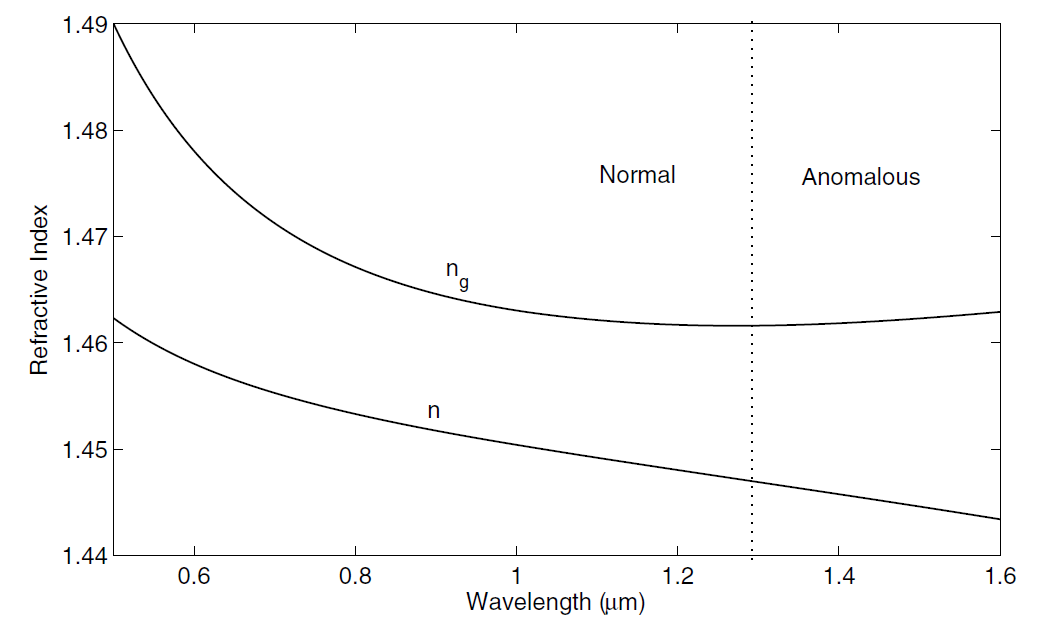
\includegraphics[width=0.6\textwidth]{images/fig1.4.PNG}
                        \caption{Variation of refractive index n and group index $n_g$ with wavelength for fused silica. $n(\omega)$ is calculated from \autoref{sellmeier equation}, $n_g(\omega)$ is calculaed from \autoref{group velocity and group index}.}
                        \label{fig1.4}
                    \end{figure}
                    
                    \begin{figure}[htbp]
                        \centering
                        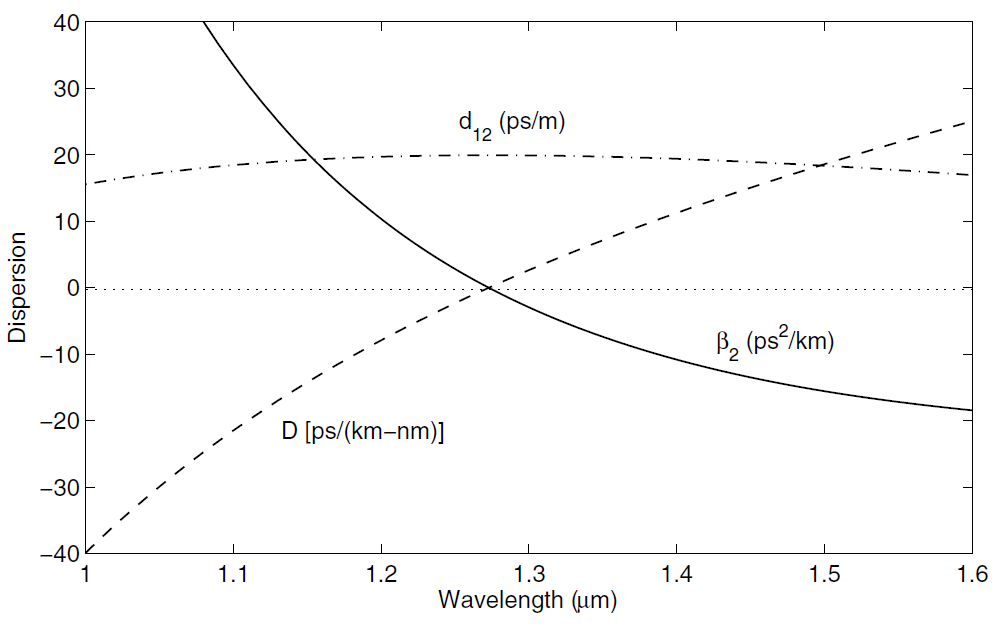
\includegraphics[width=0.6\textwidth]{images/fig1.5.PNG}
                        \caption{Variation of $\beta_2$, D, and d12 with wavelength for fused silica. Both $\beta_2$ and D vanish at the zero-dispersion wavelength($\lambda_D$) occurring near 1.27 $\mu m$. The $d_{12}$ here stands for $d_{12}(\lambda, 0.8\mu m)$ in \autoref{d12 definition}.}
                        \label{fig1.5}
                    \end{figure}
                    
                \item Zero dispersion wavelength $\lambda_D$, where $\beta_2$ and D are 0. Around this regime $\beta_3$ (Third Order Dispersion, TOD) in \autoref{propagation constant expansion} becomes important. 
                
                \item WHY $\lambda_D$ is different between bulked fused silica($1.27\mu m$) and actual glass fibers(typically $1.31\mu m$):
                    \SubItem{1.} Fiber core have dopants such as $GeO_2$ or $P_2O_5$.
                    \SubItem{2.} Fiber modes are confined in two directions, which discrete k number in these two directions. This geometry effect will influence dispersion.
                    \SubItem{3.} Other fiber design parameters such as core radius a and core-cladding index difference $\Delta$. Dispersion shift fibers can move $\lambda_D$ to $1.55\mu m$, where fiber loss at minium.
                    \SubItem{4.} dispersion-flattened optical fibers by multi-clad layer.
                    
                \item walk-off parameter $d_{12}$: nonlinear interaction between two optical pulses ceases
                to occur when the faster moving pulse completely walks through the slower moving pulse.
                    \begin{equation}
                        d_{12}(\lambda_1,\lambda_2) = \beta_1(\lambda_1)-\beta(\lambda_2) = v_g^{-1}(\lambda_1)-v_g^{-1}(\lambda_2)
                        \label{d12 definition}
                    \end{equation}
                    For pulses of width $T_0$, walk-off length $L_W$ defined by:
                    \begin{equation}
                        L_W = \frac{T_0}{\abs{d_{12}}}
                        \label{LW definition}
                    \end{equation}
            \end{itemize}
        
        
        \subsubsection{Polarization-Mode Dispersion}
            \begin{itemize}
                \item Even single mode fiber supports two degeneracy modes: x-polarization and y-polarization modes.
                \item cylindrical asymmetry and stress-induced anisotropy can break this degeneracy. This is called modal birefringence. 
                    \begin{equation}
                        B_m = \frac{\abs{\beta_x-\beta_y}}{k_0}=\abs{n_x-n_y}
                        \label{polarization birefringence definition}
                    \end{equation}
                \item For a given value of Bm, the two modes exchange their powers in a periodic fashion as they propagate inside the fiber with the Beat Length period
                    \begin{equation}
                        L_B = \frac{2\pi}{\abs{\beta_x-\beta_y}}=\frac{\lambda}{B_m}.
                        \label{Beat length definition}
                    \end{equation}
                    The intuition of Beat length can be illustrated by \autoref{beat lenghth illustration}.
                    \begin{figure}[htbp]
                        \centering
                        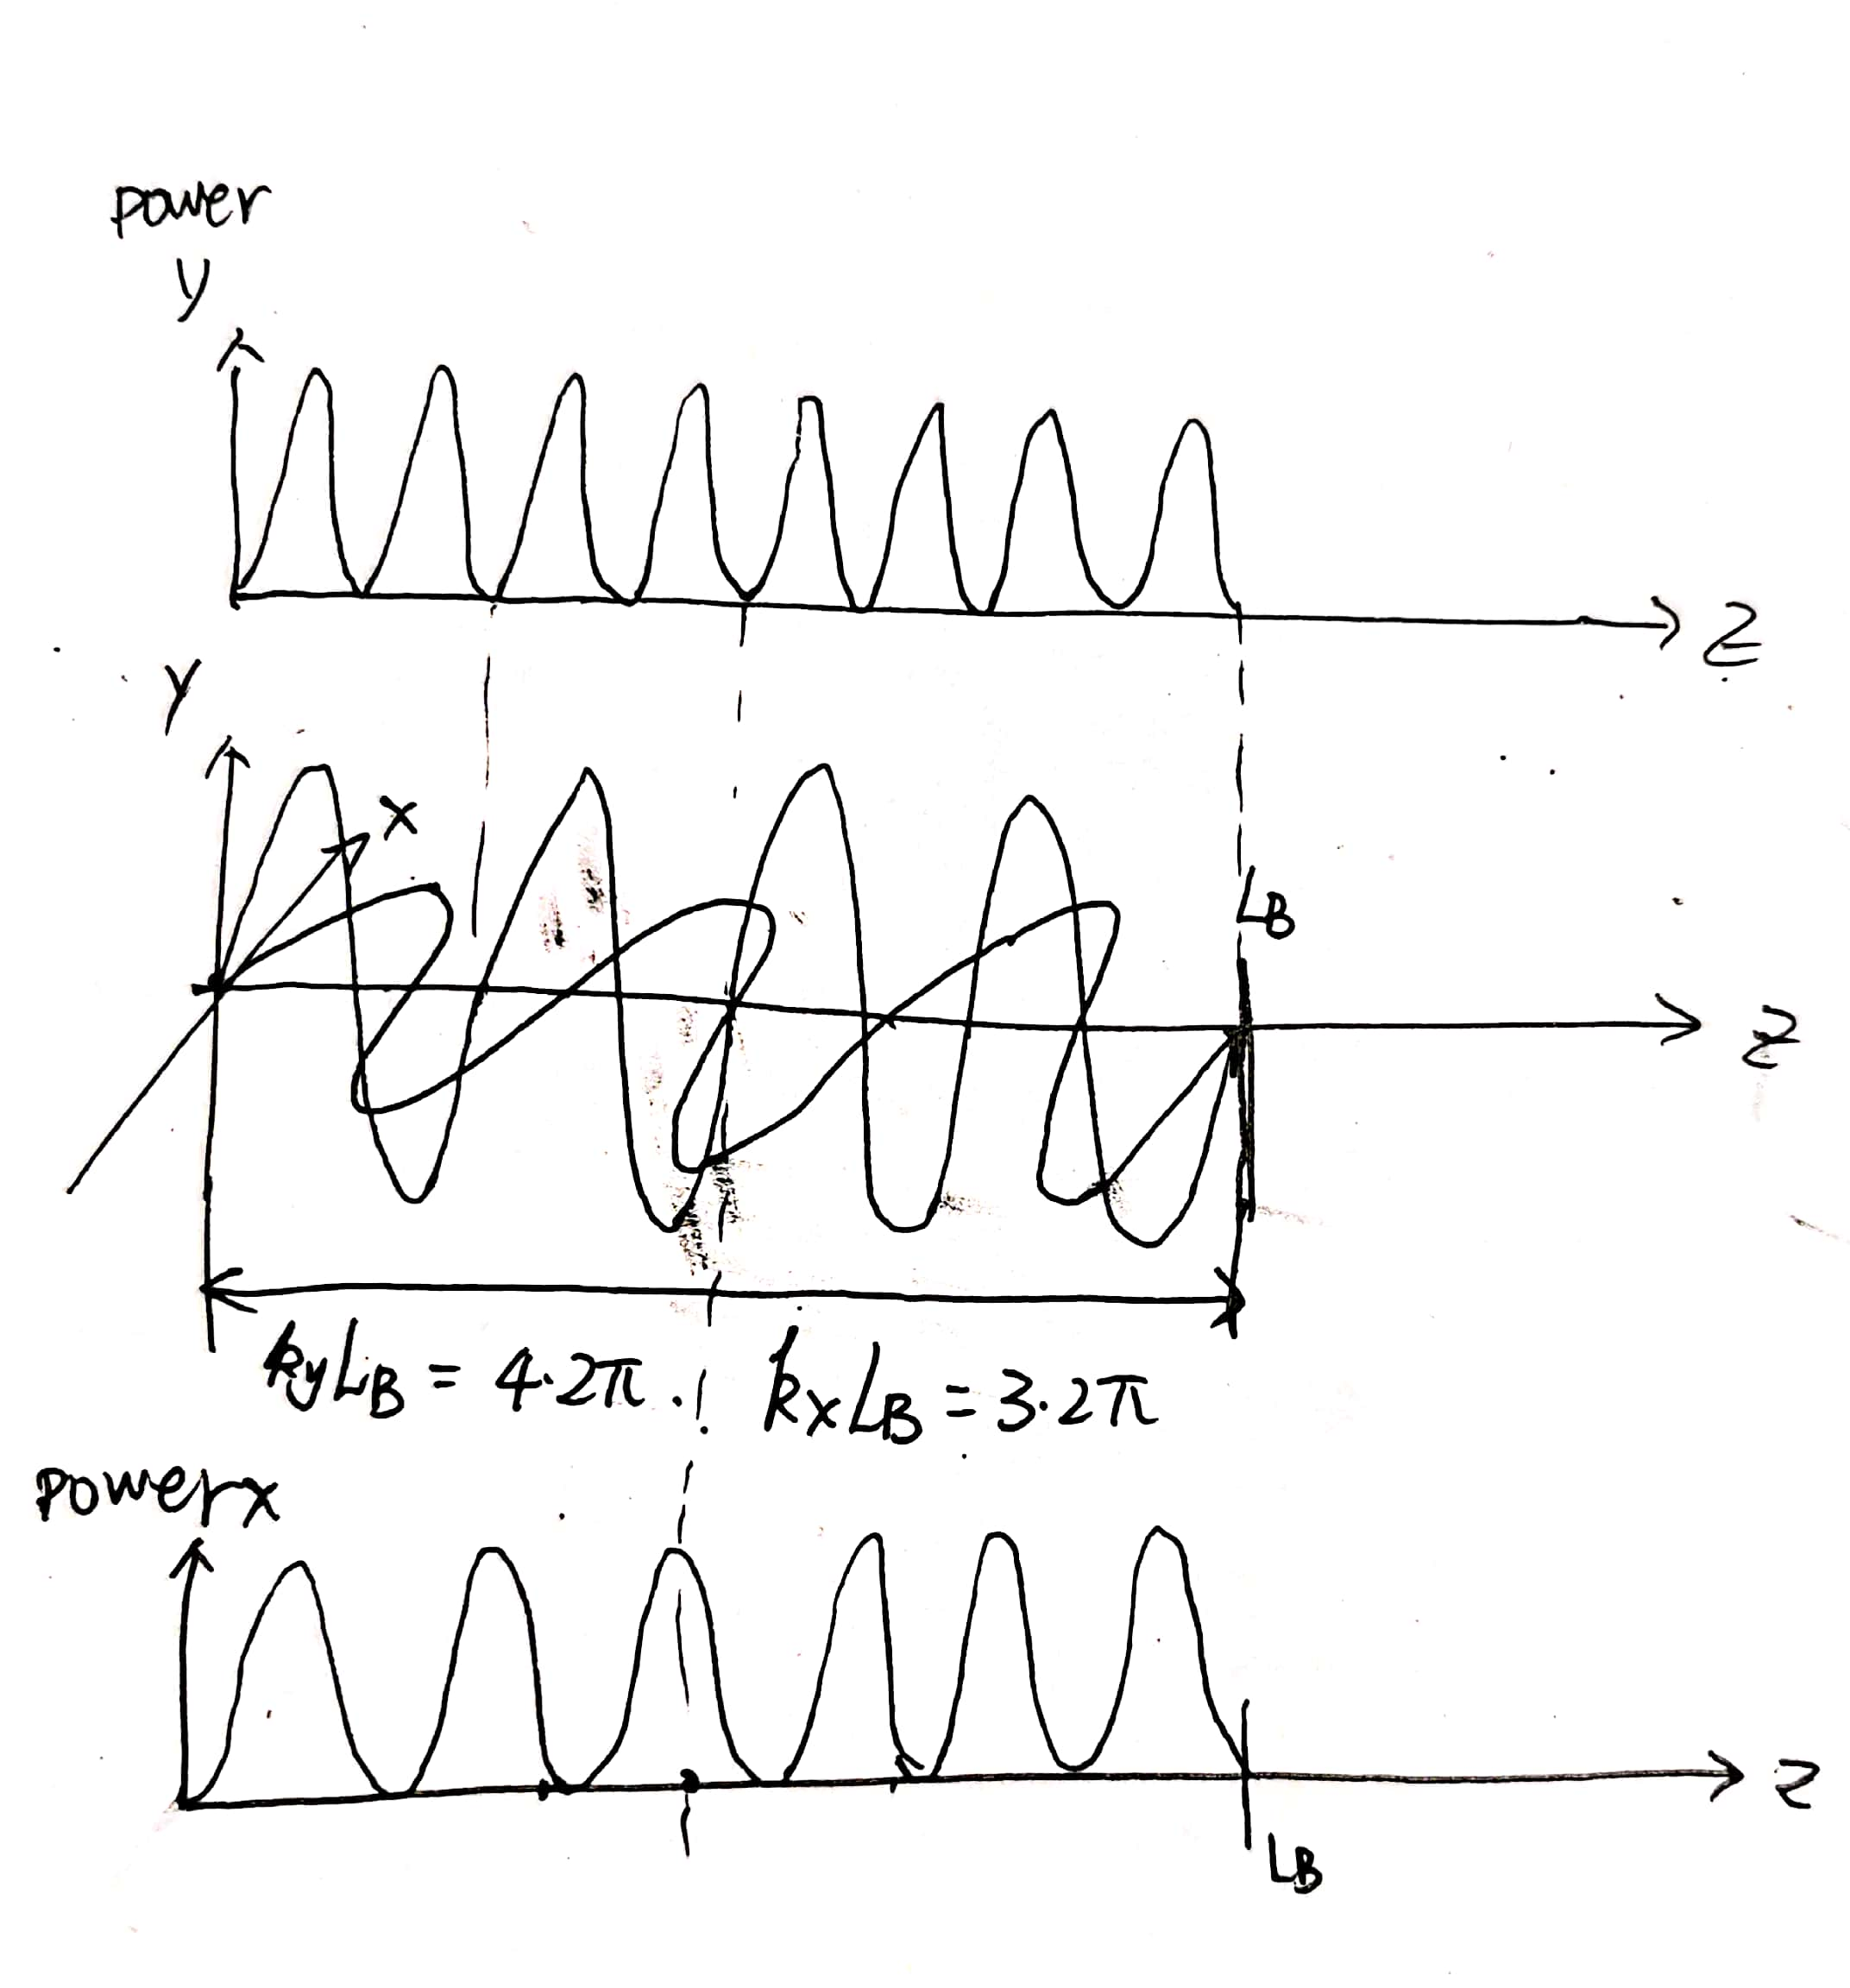
\includegraphics[width=0.6\textwidth]{images/polar_dispersion.jpg}
                        \caption{Beat length illustration}
                        \label{beat lenghth illustration}
                    \end{figure}
                    
                    \begin{figure}[htbp]
                        \centering
                        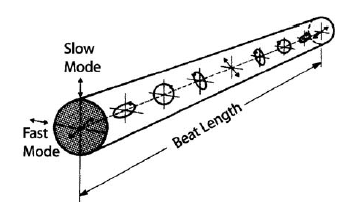
\includegraphics[width=0.6\textwidth]{images/fig1.9.PNG}
                        \caption{Evolution of state of polarization along a polarization-maintaining fiber when input signal is linearly polarized at 45 from the slow axis.}
                        \label{fig1.9}
                    \end{figure}
                    
                \item The pulse becomes broader at the output end because group velocities change $\bold{randomly}$ in response to random changes in fiber birefringence (analogous to a random-walk problem).
                    \begin{equation}
                        \Delta T = \abs{\frac{L}{v_{gx}-v_{gy}}}=L\abs{\beta_{1x}-\beta{1y}}
                    \end{equation}
                    The variance of $\Delta T$ is
                    \begin{equation}
                        \sigma_T \approx D_p \sqrt{L}.
                    \end{equation}
                    $D_p$ is PMD(Polarization-Mode Dispersion) parameter. L is travel distance.
                    
                \item polarization-maintaining fibers: induces LARGE amount of birefringence so that the FLUCTUATIONS do not significantly affect polarization.---> Which means polarization maintaining fibers can only maintain the polarization along fast or slow axis well. These fibers always called "PM fibers" or "D fibers" due to its cladding shape(See \autoref{fig1.8} inset).
                    \begin{figure}[htbp]
                        \centering
                        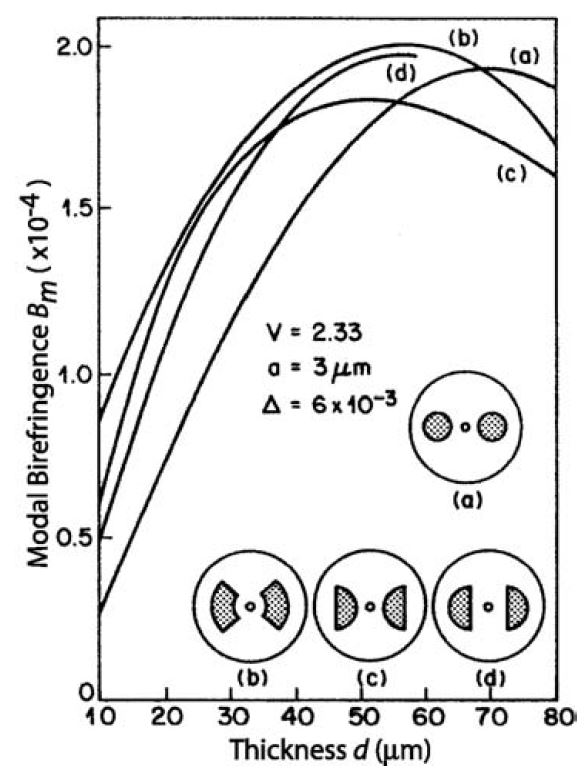
\includegraphics[width=0.6\textwidth]{images/fig1.8.PNG}
                        \caption{Variation of birefringence parameter $B_m$(See \autoref{polarization birefringence definition}) with thickness d of the stress-inducing
                        element for four different polarization-maintaining fibers. Different shapes of the
                        stress-applying elements (shaded region) are shown in the inset.}
                        \label{fig1.8}
                    \end{figure}
            \end{itemize}
            
    \subsection{Fiber Nonlinearities}
        \begin{itemize}
            \item On a fundamental level, the origin of nonlinear response is related to aharmonic motion of bound electrons under the influence of an applied field.
            \item Generally two types of nonlinearity are important in silica nonlinear medium. 
                \SubItem{The first type doesn't energy exchange between optical fields and the medium, which can be described in the language of electrical polarization (\autoref{general PE relation}) and refractive index (\autoref{n2 bar relation with chi3}).}
                \SubItem{The second type includes energy exchange between optical field and medium, which is called inelastic scattering process. The phonons induced by this process can be in optical (SRS) or acoustic (SBS).}
            \item Total polarization P induced by electric dipoles is not linear in the electric field E, but satisfies the more general relation:
                \begin{equation}
                    \frac{\boldsymbol{P}}{\epsilon_0} = \chi^{(1)} \cdot \boldsymbol{E} + \chi^{(2)} : \boldsymbol{EE} + \chi^{(3)} \vdots \boldsymbol{EEE} + \dots,
                    \label{general PE relation}
                \end{equation}
                where $\chi^{(j)}$ is jth order susceptibility. 
                \SubItem{Take special notice of the relation between \autoref{sellmeier equation} and \autoref{general PE relation}. In \autoref{sellmeier equation}, no nonlinearity is considered, only dispersion is considered. Thus \autoref{sellmeier equation} is correlated with the first term in \autoref{general PE relation}. which means:
                    \begin{equation}
                        \frac{\boldsymbol{P}}{\epsilon_0} = \chi^{(1)}(\omega) \cdot \boldsymbol{E} \iff n(\omega).
                    \end{equation}
                    The high order terms in \autoref{general PE relation} are not related with \autoref{sellmeier equation} since they are nonlinear terms. \autoref{sellmeier equation} don't show the power dependence of refractive index.
                }
                \SubItem{In general, $\chi^{(j)}$ is a (j,1)-tensor\cite{noauthor_tensor_2019} of rank j+1. The reason it is (j,1)-tensor is that this is a "mapping" coefficient taking in j-copies of 3-dim Cartesian space(i.e.$\boldsymbol{EE\dots}$) into a 1-cpoy of 3-dim Cartesian space(i.e. $\boldsymbol{P}$). (It might be useful to refer to \autoref{fig: chi1 and chi3 freq domain illustration} to understand better.)}
                \SubItem{ Rank 4 tensor is a good example to illustrate the difference between convariant and contravariant indexes. Any tensor is a (p,q)-tensor with rank of p+q, where p is contravariant index, denoted as the uppper index; q is covariant index, denoted as lower index.
                    \begin{itemize}
                        \item For rank-4 tensors, typically have two types: type (3,1), such as 3rd order susceptibility $\chi^{(3)}$; and type (2,2), such as elasticity tensor\cite{noauthor_hookes_2019}.
                        \item For rank 4 type (3,1): 3rd order susceptibility $\chi^{(3)}$, has 3 contravariant index(upper index) and 1 covariant index(lower index). The mathematical formation of $\chi^{(3)}$ is
                            \begin{equation}
                                \label{illustration of chi3 as (1,3)-tensor}
                                \frac{\boldsymbol{P}^{(3)}}{\epsilon_0} = \chi^{(3)} \vdots \boldsymbol{EEE}.
                            \end{equation}
                        Expand $\boldsymbol{P}^{(3)}$ in x,y,z directions (Using Einstein summation notation, sum over same notations, which are $ ijk \in \{x,y,z\} $ here):
                            \begin{equation}
                                \begin{cases}
                                P^{(3)}_x /\epsilon_0 = {\chi^{(3)}}_x^{ijk}E_i E_j E_k\\
                                P^{(3)}_y / \epsilon_0 = {\chi^{(3)}}_y^{ijk}E_i E_j E_k\\
                                P^{(3)}_z /\epsilon_0 = {\chi^{(3)}}_z^{ijk}E_i E_j E_k.
                                \end{cases}
                            \end{equation}
                        Thus $\chi^{(3)}$ is type (3,1) rank 4-tensor with 3 contravariant indexes and 1 covariant index.
                        \item For rank 4 type (2,2): elasticity tensor $\boldsymbol{c}$ \cite{noauthor_hookes_2019}, relates strain tensor $\boldsymbol{\epsilon}$ (in lieu of the displacement X in F=-kX) and the stress tensor $\boldsymbol{\sigma}$ (replacing the restoring force F) as
                            \begin{equation}
                                \boldsymbol{\sigma} = - \boldsymbol{c} \boldsymbol{\epsilon},
                                \label{Hooke's law in tensor form}
                            \end{equation}
                            where strain tensor $\boldsymbol{\epsilon}$ and stress tensor $\boldsymbol{\sigma}$ are order 2 tensor with 3-dim.
                                \begin{multicols}{2}
                                \setlength{\columnseprule}{0pt}
                                \noindent
                                    \begin{equation}
                                        \boldsymbol{\epsilon} = 
                                            \begin{pmatrix}
                                                \epsilon_{xx} & \epsilon_{xy} & \epsilon_{xz}\\
                                                \epsilon_{yx} & \epsilon_{yy} & \epsilon_{yz}\\
                                                \epsilon_{zx} & \epsilon_{zy} & \epsilon_{zz}
                                            \end{pmatrix}
                                    \end{equation}
                                    \begin{equation}
                                        \boldsymbol{\sigma} = 
                                            \begin{pmatrix}
                                                \sigma_{xx} & \sigma_{xy} & \sigma_{xz}\\
                                                \sigma_{yx} & \sigma_{yy} & \sigma_{yz}\\
                                                \sigma_{zx} & \sigma_{zy} & \sigma_{zz}
                                            \end{pmatrix}.
                                    \end{equation}
                                \end{multicols}
                            The relation between $\boldsymbol{\epsilon}$ and $\boldsymbol{\sigma}$ is connected by $\boldsymbol{c}$ in the form of
                                \begin{equation}
                                    \sigma_{ij} = {c_{ij}}^{kl}\epsilon_{kl},
                                \end{equation}
                            where common indexes to sum up are $ kl \in \{x,y,z\} $ this time. \\
                            Thus $\boldsymbol{c}$ is type (2,2) rank 4-tensor with 2 contravariant indexes and 2 covariant indexes.
                    \end{itemize}
                }
            \item second-order susceptibility: second-harmonic generation; sum-frequency generation. nonzero only for media that lack an inversion symmetry at the molecular level. 
                \SubItem{Silica doesn't have this in-symmetry. Only electric-quadrupole and magnetic-dipole moments can generate weak second-order nonlinear effects. Defects or color centers inside the fiber core can also contribute to second-harmonic generation.}
            \item third-order susceptibility: third-harmonic generation; four-wave mixing; nonlinear refraction.
                \SubItem{Unless special efforts are made to achieve \textbf{phase matching}, the nonlinear processes that involve generation of new frequencies (e.g., third-harmonic generation and four-wave mixing) are not efficient in optical fibers.\label{Why nonlinear refraction most important} }
        \end{itemize}
        
        \subsubsection{Nonlinear Refraction}
            \begin{itemize}
                \item As \ref{Why nonlinear refraction most important} said, silica fiber doesn't have second order nonlinearity, thus refractive index in the simplest form is (\MakeUppercase{Note: optical intensities I has the units of $W/m^2$}):
                    \begin{equation}
                        \Tilde{n}(\omega,I) = n(\omega) + n_2^I I = n(\omega) + \overline{n}_2\abs{\boldsymbol{E}}^2,
                        \label{simplest nonlinear refractive index form}
                    \end{equation}
                    which is isotropic(This is very important!). In \autoref{simplest nonlinear refractive index form}, $n(\omega)$ is the linear part (This linear doesn't mean Taylor expansion to 1st order, this linear means a linear process, which refractive index has no relation with electric field) given by \autoref{sellmeier equation}. $\overline{n}_2$ is the average $n_2$ over fiber cross-section. Notice $\abs{\boldsymbol{E}}^2$ also evolves some kind of average over the fiber cross-section.
                \item Because $I=\frac{1}{2}\epsilon_0 c n \abs{\boldsymbol{E}}^2$, $n_2$ and $n_2^I$ are related by:
                    \begin{equation}
                        \label{n2 and n2I relation}
                        n_2^I = \frac{2n_2}{\epsilon_0 c n}
                    \end{equation}
                \item $\overline{n}_2$ is nonlinear index coefficient, related to  $\chi^{(3)}$ by (will be derived later)
                    \begin{equation}
                        \overline{n}_2 = \frac{3}{8n} \Re({{ \chi^{(3)} }_x}^{xxx}).
                        \label{n2 bar relation with chi3}
                    \end{equation}
                    Notice that optical field E is assumed to be linearly polarized so that only one component ${ \chi^{(3)} }_x^{xxx}$ contributes. Other components can affect polarization by nonlinear birefringence.
                \item Self-phase modulation (SPM): Self induced phase shift during its propagation through nonlinear fibers. Total propagation phase is
                    \begin{equation}
                        \phi = \Tilde{n}k_0 L = (n+\overline{n}_2\abs{\boldsymbol{E}}^2)k_0 L .
                        \label{SPM propagation phase}
                    \end{equation}
                    This can be simply understood by refractive index shift due to light intensity. \MakeUppercase{However this simple understanding does not applies Cross-phase modulation situation!}
                \item Cross-phase modulation (XPM): Involves two(or more) frequency components, optical fields can be expressed by
                    \begin{equation}
                        \boldsymbol{E} = \frac{1}{2} \boldsymbol{\hat{x}}[E_1\exp{-i\omega_1t} + E_2\exp{-i\omega_2 t} + c.c.] ,
                        \label{two mode optical field}
                    \end{equation}
                    $\boldsymbol{\hat{x}}$ is polarization direction. The nonlinear phase shift is given by
                    \begin{equation}
                        \phi_{NL} = \overline{n}_2 k_0 L(\abs{E_1}^2+2\abs{E_2}^2).
                        \label{cross phase modulation NL phase shift}
                    \end{equation}
                Special notice that for equally intense optical fields of differnet frequency components, \MakeUppercase{XPM is twice that of SPM}. This can not be intuitively derived from \autoref{SPM propagation phase}. Instead this should be understood intuitively from \autoref{general PE relation}. From \autoref{general PE relation}, the nonlinear part of propagation phase is induced by term
                \begin{equation}
                    \boldsymbol{P}^{(3)} = \epsilon_0 \chi^{(3)} \vdots \boldsymbol{EEE},
                \end{equation}
                which can be generally understood to be proportional to cubed E, $\abs{\boldsymbol{E}}^3$. From \autoref{two mode optical field}, $\abs{\boldsymbol{E}}^3$ can be expressed as
                \begin{equation}
                    \begin{split}
                        \abs{\boldsymbol{E}}^3 =& \frac{1}{8}(E_1\exp{-i\omega_1 t} + E_2\exp{-i\omega_2 t} + E_1^*\exp{i\omega_1 t} + E_2^*\exp{i\omega_2 t})^3\\
                        =&\frac{1}{8} [E_1\exp{-i\omega_1t}(3\abs{E_1}^2+6\abs{E_2}^2) +E_2\exp{-i\omega_2t}(3\abs{E_2}^2+6\abs{E_1}^2) \\ & +\dots].
                    \end{split}
                    \label{cube of two mode optical field}
                \end{equation}
                Only freq components at $\exp{-i\omega_1t}$ and $\exp{-i\omega_2t}$ is on resonance with the optical field, and contributes to XPM refractive index. From \autoref{cube of two mode optical field} we have a rough derivation of where does the twice in \autoref{cross phase modulation NL phase shift} comes from. However more detailed derivation (including \autoref{n2 bar relation with chi3}) should originate from Maxwell equation and wave propagation equation, which will be included in the following chapter.
            \end{itemize}
        \subsubsection{Stimulated Inelastic Scattering}
            \begin{itemize}
                \item Vibrational excitation modes stimulated by electromagnetic field in silica, this process is called stimulated inelastic scattering.
                \item Scattering annihilated a photon of incident field (called pump), create a photon at lower frequency (belonging to Stokes wave) and a phonon to conserve energy and momentum. Some time higher frequency photon can also be generated (belonging to anti-Stokes wave).
                \item Stimulated Raman scattering (SRS), induces optical phonons in  medium, can occur in both directions. Stimulated Brillouin scattering, occurs only in backward direction.
                \item The initial growth of Stokes wave can be described by
                    \begin{multicols}{2}
                    \setlength{\columnseprule}{0pt}
                    \noindent
                        \begin{equation}
                            \dv{I_s}{z} = g_R I_p I_s,
                        \end{equation}
                        \begin{equation}
                            \dv{I_s}{z} = g_B I_p I_s.
                        \end{equation}
                    \end{multicols}
                    $I_s$ is Stokes intensity, $I_p$ is pump intensity (both have units of $W/m^2$). $g_R$ and $g_B$ are Raman-gain coefficient and Brillouin-gain coefficient. The gain coefficient spectrum are always described by pump-Stokes line detuning. 
                    \begin{figure}[htbp]
                        \centering
                        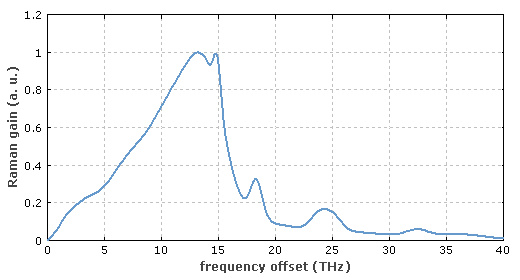
\includegraphics[width=0.6\textwidth]{images/raman_gain.png}
                        \caption{Raman gain spectrum of silica, as used e.g. in silica fibers. The quantity on the horizontal axis is the frequency offset of the signal wave with respect to the pump wave.\cite{hollenbeck_multiple-vibrational-mode_2002, paschotta_raman_nodate}}
                        \label{raman gain spectrum figure}
                    \end{figure}
                \item Gain bandwidth:
                    \SubItem{Raman-gain spectrum is very broad band(optical phonons), peak gain $g_R \approx 6 \times 10^{-14} m/W$ at pump near $1.5 \mu m$ with a spectral shift about 13.1THz.} \SubItem{Brillouin-gain spectrum is very narrow band (<100MHz, acoustic phonons), peak gain $g_B \approx 6 \times 10^{-11} m/W$ at pump near $1.5 \mu m$ with a spectral shift about 10GHz. Also $g_B$ decreases by a factor of $\Delta \nu_p/\Delta \nu_B$ for a broad-bandwidth pump. $\Delta \nu_p$ is pump bandwidth and $\Delta \nu_B$ is Brillouin-gain bandwidth.} 
                \item Threshold behavior:
                    \SubItem{For SRS in a single mode fiber, with $\alpha \gg 1$ ($\alpha$ see \autoref{attenuation constant}), which means pump power is almost attenuated to 0 and leav only Raman lines. A threshold pump intensity is given by \cite{smith_optical_1972}
                    \begin{equation}
                        I_P^{th} \approx 16(\frac{\alpha}{g_R}).
                    \end{equation}
                    Typically $I_P^{th} \approx 10mW/cm^2$, SRS can be observed at a pump power $\approx 1W$.
                    }
                    \SubItem{Similar to SRS, SBS threshold is given by\cite{smith_optical_1972}
                    \begin{equation}
                        I_p^{th} \approx 21(\frac{\alpha}{g_B}).
                    \end{equation}
                    As gain efficient differs nearly three orders, typical SBS threshold are $\approx 1mW$.
                    }
            \end{itemize}
        \subsubsection{Importance of Nonlinear Effects}
             \begin{itemize}
                 \item Typical $n_2$ in silica fiber yield in range of $2.2-3.4 \times 10^{-20} m^2/W$, which is at least 2-order smaller than other nonlinear medium.
                 \item Two factors contributed to the enhancement:
                    \SubItem{Small spot size $\< 10\mu m$.}
                    \SubItem{Low loss $<1dB/km$ in wavelength $1.0-1.6 \mu m$.}
                    
                    These two factors dramatically enhanced the effective interaction length. In bulked silica, interaction length is considered to be related to light focal region $\approx \pi w_0^2/\lambda$. However in fiber the whole transmission length can be considered to be effective interaction length.
             \end{itemize}
    \subsection{Overview}
        \begin{itemize}
            \item Chapter 1-3: background and mathematical tools.
                \SubItem{Chapter 2: Mathematical framework starting from Maxwell's equation. Including important approximations and numerical methods.}
                \SubItem{Chapter 3: Group velocity Dispersions (GVD, see \autoref{beta2 definition}) when incident power and fiber length are such that nonlinear effect are negligible. GVD (temporal broadening) and effects of frequency chirp. High order effects near $\lambda_D$ (See \autoref{fig1.5}).}
            \item Chapter 4-7: Non-scattering nonlinear effects and its spectral and temporal effects.
                \SubItem{Chapter 4: SPM (Self-phase modulation), causes spectrum broadening. Pulse shape also affected when GVD and SPM affects together.}
                \SubItem{Chapter 5: Optical Solitons. Modulation instability due to the interplay of GVD and nonlinear effects in anomalous-GVD (See \autoref{Summary of normal and anomalous dispersion}) regime. Topics includes: High order solitons, inverse scattering method to solve nonlinear Schrodinger equation; Dark solitons; Soliton decay related to higher-order nonlinear and dispersive effects.}
                \SubItem{Chapter 6-7: XPM. Chapter 6 focus on XPM between orthogonally polarized components. Included optical Kerr effect and birefringence-induced pulse shaping. Chapter 7 foucs on XPM between different wavelengths, XPM-interaction lead to modulation instability even in normal-GVD regime. Asymmetric spectral and temporal changes when consider XPM, SPM and GVD together. XPM-interaction between counterpropagating waves, which is important in gyroscopes.}
            \item Chapter 8-12: Nonlinear effects generate new optical wavelengths.
                \SubItem{Chapter 8: SRS. Raman gain and Raman threshold. SRS for CW wave and short pulse. Some features are leaded with conbination of SPM, XPM, GVD. And significantly different for normal-GVD and anormalous-GVD (fiber-Raman soliton lasers). Polariaztion effects.}
                \SubItem{Chapter 9: SBS. Transfer energy only to counterpropagating Stokes wave. Only when CW or pulse spectral width smaller than Brillouin bandwidth. Effects including: Brillouin threshold, pump depletion, gain saturation; Fiber-based Brillouin amplifiers; Brillouin fiber lasers.}
                \SubItem{Chapter 10: FWM (Four-wave mixing). This can efficiently occur only when phase matched. Phase-matching technique; Parametric amplification; Polariaztion effects.}
                \SubItem{Chapter 11-12: Highly-nonlinear fibers. Chapter 11 introduces techniques to measure fiber parameters and four types of highly nonlinear fibers. Chapter 12 discussed intrapulse Raman scattering and FWM, supercontinuum generation, second- and third-harmonic generation.}
        \end{itemize}

\newpage
\section{Pulse Propagation in Fibers}
    \subsection{Maxwell's Equations}
        Simply reminder, Maxwell equation in medium (NOT necessary linear) is:
        \begin{subequations}
        \label{Maxwell's equation}
            \begin{align}
                &\boldsymbol{\bigtriangledown} \times \boldsymbol{E} = -\pdv{\boldsymbol{B}}{t} \label{Maxwell equation: cor E} \\
                &\boldsymbol{\bigtriangledown} \times \boldsymbol{H} = \boldsymbol{J} + \pdv{\boldsymbol{D}}{t} \label{Maxwell equation: cor H}\\
                &\boldsymbol{\bigtriangledown} \cdot \boldsymbol{D} = \rho_f \label{Maxwell equation: div D}\\
                &\boldsymbol{\bigtriangledown} \cdot \boldsymbol{B} = 0 \label{Maxwell equation: div B}
            \end{align}
        \end{subequations}
        In free charge absent medium, $\rho_f=0$, $\boldsymbol{J}=\boldsymbol{0}$. $\boldsymbol{D}$ and $\boldsymbol{B}$ are related with $\boldsymbol{E}$ and $\boldsymbol{H}$ by constitutive relations
        \begin{subequations}
            \label{Medium electric relations}
            \begin{align}
                \boldsymbol{D} &= \epsilon_0 \boldsymbol{E} + \boldsymbol{P}, \label{medium electric: D, E, P}\\
                \boldsymbol{B} &= \mu_0 \boldsymbol{H} + \boldsymbol{M}. \label{medium electric: B, H, M}
            \end{align}
        \end{subequations}
        In nonmagnetic medium, $\boldsymbol{M}=\boldsymbol{0}$.\\
        Propagation equation can be derived from Maxwell's equation \autoref{Maxwell equation: cor E}, \autoref{Maxwell equation: div D} and \autoref{medium electric: D, E, P}.\\
            \begin{equation}
                \Lap \times (\Lap\times\boldsymbol{E}) = -\frac{1}{c^2}\pdv[2]{\boldsymbol{E}}{t}-\mu_0\pdv[2]{\boldsymbol{P}}{t}
            \end{equation}
        For nonlinear version, $\boldsymbol{P} = \boldsymbol{P_L}+\boldsymbol{P_{NL}}$:
            \begin{equation}
                \Lap \times (\Lap\times\boldsymbol{E}) = -\frac{1}{c^2}\pdv[2]{\boldsymbol{E}}{t}-\mu_0\pdv[2]{\boldsymbol{P_L}}{t}-\mu_0\pdv[2]{\boldsymbol{P_{NL}}}{t}
                \label{propagating equation of E with PL and PNL: including laplace symbol}
            \end{equation}
            
        % \MakeUppercase{Note that in the second equal of} \autoref{medium electric: D, E, P}, \MakeUppercase{Linear medium is required. As long as $\epsilon$ is written, linear medium is required.}  Remind that we used to write $\epsilon = 1 + \chi$, when we were dealing with linear medium.\\
        
        Usually $P_{NL}$ is treated as perturbation. Thus since now we consider linear situation, which is the basis of Nonlinear perturbation.
            \begin{equation}
                \begin{split}
                    \Lap \times (\Lap\times\boldsymbol{E}) &= -\frac{1}{c^2}\pdv[2]{\boldsymbol{E}}{t}-\mu_0\pdv[2]{\boldsymbol{P}}{t}\\
                    &=-\frac{\epsilon}{c^2}\pdv[2]{\boldsymbol{E}}{t}
                \end{split}
                \label{Propagation E equation: E and P}
            \end{equation}
        Remind that we write $\epsilon = 1 + \chi$, when we were dealing with linear medium, $\boldsymbol{D} = \epsilon\epsilon_0\boldsymbol{E}$. Rewrite \autoref{Propagation E equation: E and P} in frequency domain, (In fact this is an Laplace transformation)
            \begin{subequations}
                \label{E in time domain and frequency domain}
                \begin{align}
                    \Tilde{\boldsymbol{E}}(\boldsymbol{r},\omega) &= \int_{-\infty}^{\infty} \boldsymbol{E}(\boldsymbol{r},t)\exp{i\omega t}dt\label{From E in time domain to E in freq domain},\\
                    \boldsymbol{E}(\boldsymbol{r},t) &=\frac{1}{2\pi} \int_{-\infty}^{\infty} \Tilde{\boldsymbol{E}}(\boldsymbol{r},\omega)\exp{-i\omega t}d\omega ,\label{From E in freq domain to E in time domain}
                \end{align}
            \end{subequations}
        we can get (Basically is to change $\partial_t$ to $i\omega$):
            \begin{equation}
                \Lap^2\Tilde{\boldsymbol{E}}+\epsilon(\omega)\frac{\omega^2}{c^2}\Tilde{\boldsymbol{E}}=0.
                \label{Propagation E equation in freq domain}
            \end{equation}
        Used relation:
            \begin{equation}
                \Lap\times(\Lap\times\boldsymbol{E})=\Lap(\Lap\cdot\boldsymbol{E})-\Lap^2\boldsymbol{E}=-\Lap^2\boldsymbol{E}.
                \label{double crossing laplace relation}
            \end{equation}
        The definition of $\epsilon$ is
            \begin{equation}
                \epsilon = (n + \frac{i\alpha c}{2\omega})^2
                \label{relation between epsilon, n and alpha}
            \end{equation}
        when dispersion and attenuation is evolved. $\alpha$ is the attenuation constant in \autoref{attenuation constant}. When $\alpha$ is small enough, \autoref{Propagation E equation in freq domain} can also be written as
            \begin{equation}
                \label{Propagation E equation in freq domain: small attenuation circumstance}
                \Lap^2\Tilde{\boldsymbol{E}}+n^2(\omega)\frac{\omega^2}{c^2}\Tilde{\boldsymbol{E}}=0.
            \end{equation}
        Also, $\epsilon(\omega)=1+\Tilde{\chi}^{(1)}(\omega)$, using \autoref{relation between epsilon, n and alpha} and an approximation of $\frac{\alpha^2c^2}{4\omega^2}+\Re{\chi^{(1)}} \ll 1$, we can get
            \begin{subequations}
                \begin{align}
                    n(\omega) &= 1+\frac{1}{2}\Re{\Tilde{\chi^{(1)}}},\\
                    \alpha(\omega) &=\frac{\omega}{nc}\Im{\Tilde{\chi^{(1)}}}.
                \end{align}
            \end{subequations}
        The same procedure of getting \autoref{Propagation E equation in freq domain: small attenuation circumstance} can be done to $\Tilde{\boldsymbol{H}}$,
            \begin{equation}
                \label{Propagation H equation in freq domain: small attenuation circumstance}
                \Lap^2\Tilde{\boldsymbol{H}}+n^2(\omega)\frac{\omega^2}{c^2}\Tilde{\boldsymbol{H}}=0.
            \end{equation}
            
    \subsection{Fiber Modes}
        \subsubsection{Eigenvalue Equation}
            \begin{itemize}
                \item \autoref{Propagation E equation in freq domain: small attenuation circumstance} in cylindrical coordinates $\rho,\phi,z$ is
                    \begin{equation}
                        \pdv[2]{\Tilde{\boldsymbol{E}}}{\rho}+\frac{1}{\rho}\pdv{\Tilde{\boldsymbol{E}}}{\rho}+\frac{1}{\rho^2}\pdv[2]{\Tilde{\boldsymbol{E}}}{\phi}+\pdv[2]{\Tilde{\boldsymbol{E}}}{z}+n^2k_0^2\Tilde{\boldsymbol{E}}=0.
                        \label{maxwell equation in cylindrical coordinates}
                    \end{equation}
                \item $\Tilde{\boldsymbol{E}}$ and $\Tilde{\boldsymbol{H}}$ each contains 3 dimensions of components($\Tilde{E_Z}$, $\Tilde{E_\rho}$, $\Tilde{E_\phi}$; $\Tilde{H_Z}$, $\Tilde{H_\rho}$, $\Tilde{H_\phi}$). These 6 components satisfies 4 equations in \autoref{Maxwell's equation}. Thus only two components of 6 are independent, choose $\Tilde{E_z}$ and $\Tilde{H_z}$. 
                
                \item Separation of variables:
                    \begin{equation}
                        \Tilde{E_z} = A(\omega)F(\rho)\exp{im\phi}\exp{i\beta z}.
                    \end{equation}
                    $\beta$ is propagation constant, $m$ is an integer. $F(\rho)$ is the solution of
                    \begin{equation}
                        \dv[2]{F}{\rho} + \frac{1}{\rho}\dv{F}{\rho}+(n^2k_0^2-\beta^2-\frac{m^2}{\rho^2})F=0
                        \label{Equation F of rho satisfies}
                    \end{equation}
                    \SubItem{For $\rho < a$, a is core radius:
                        \begin{equation}
                            \begin{split}
                                F(\rho)&=C_1 J_m(p\rho)+C_2 N_m(p\rho).\\
                                p &= \sqrt{n_1^2k_0^2-\beta^2}
                                \label{Electric mode in the core}
                            \end{split}
                        \end{equation}
                        $J_m(p\rho)$ and $N_m(p\rho)$ are Bessel and Neumann function respectively. Requiring $n_1^2k_0^2-\beta^2 > 0$. To avoid singularity at $\rho = 0$, $C_2 = 0$ required for a physically meaningful solution.
                    }
                    \SubItem{For $\rho > a$, a is core radius:
                        \begin{equation}
                            \begin{split}
                                F(\rho)&=K_m(q\rho).\\
                                q &= \sqrt{\beta^2-n_c^2k_0^2}
                                \label{Electric mode in the cladder}
                            \end{split}
                        \end{equation}
                        $K_m(q\rho)$ is the second type of virtual scalar Bessel function. Requiring $n_c^2k_0^2-\beta^2 < 0$}. (This choice aims for exponential decay along $\rho$ direction.)
                \item Eigenvalue equation: from the tangential components continuous of $\Tilde{E_Z}$, $\Tilde{E_\phi}$; $\Tilde{H_Z}$, $\Tilde{H_\phi}$, we get eigenvalue $\beta$ equation:
                    \begin{equation}
                        [\frac{J_m^{'} (pa)}{pJ_m(pa)}+\frac{K_m^{'} (qa)}{qK_m(qa)}][\frac{J_m^{'} (pa)}{pJ_m(pa)}+\frac{n_c^2}{n_1^2}\frac{K_m^{'} (qa)}{qK_m(qa)}]=(\frac{m\beta k_0(n_1^2-n_c^2)}{an_1 pq})^2.
                        \label{eigen value equation of beta}
                    \end{equation}
                    Each m has a series of solution $\beta_mn$. Each $\beta_mn$ corresponds to a mode. See derivations in Chapter 2 of \cite{marcuse_theory_1991}.
                \item Cut off freq: According to \autoref{Electric mode in the core} and \autoref{Electric mode in the cladder}, we get
                    \begin{equation}
                        p^2+q^2=(n_1^2-n_c^2)k_0^2.
                        \label{equation to solve cut off freq}
                    \end{equation}
                    Cut off freq is determined by $p_c$ when q = 0. Define V as \autoref{V parameter}. For single mode fiber, $V<V_c$ then all modes except $HE_{11}$ mode are cut off. where $V_c$ is the smallest solution of $J_0(V_c)=0$, or $V_c\approx 2.405$.
                \item Example: If $n_1-n_c=0.005$, $a=4\mu m$, from \autoref{equation to solve cut off freq} we can get $\lambda_c=1.2\mu m$ ($k_0=2\pi/\lambda_c$).Such fiber supports single mode only when $\lambda>\lambda_c=1,2\mu m$. To support single mode in visible region, typically $a<2\mu m$.
             \end{itemize}
        \subsubsection{Characteristics of the Fundamental Mode}
            \begin{itemize}
                \item Single mode fiber supports only $HE_11$ mode, which has three non-zero components $\Tilde{E_\rho}$, $\Tilde{E_\phi}$; $\Tilde{E_Z}$. Either x- or y- are leading part. Two poliarization parts are contained.
                \item $LP_{mn}$ denotes linear poliazed modes, which are APPROXIMATE solutions of \autoref{maxwell equation in cylindrical coordinates}.  $HE_{11}$ corresponds to $LP_{01}$.
                \item Give $LP_{11}$ as 
                    \begin{equation}
                        \Tilde{\boldsymbol{E}}(\boldsymbol{r},\omega) = \hat{x}{A(\omega)F(x,y)\exp{i\beta(\omega)z}}.
                    \end{equation}
                    \SubItem{For $\rho<a$, ($\rho=\sqrt{x^2+y^2}$)
                        \begin{equation}
                            F(x,y)=J_0(p\rho)
                            \label{fundamental electric mode in core}
                        \end{equation}
                    }
                    \SubItem{For $\rho>a$, Take the approximation of $K_m(q\rho)$ in \autoref{Electric mode in the cladder}, and  a constant factor to ensure the equality of F at $\rho=a$, we get
                        \begin{equation}
                            F(x,y)=\sqrt{\frac{a}{\rho}}J_0(pa)\exp{-q(\rho-a)}.
                            \label{fundamental electric mode in cladder}
                        \end{equation}
                    }
                \item A good approximation of \autoref{fundamental electric mode in core} and \autoref{fundamental electric mode in cladder} is a Gaussian function:
                    \begin{equation}
                        F(x,y)=\exp{-\frac{x^2+y^2}{w^2}},
                    \end{equation}
                    The fitting can be seen on right plot of \autoref{fig2.1}. w is related with V (\autoref{V parameter}) by a fitting:
                    \begin{equation}
                        \frac{w}{a} \approx 0.65+1.619V^{-1.5}+2.879V^{-6}.
                    \end{equation}
                    The plot of w(V) can be seen at left plot of \autoref{fig2.1}.
                    \begin{figure}[htbp]
                        \centering
                        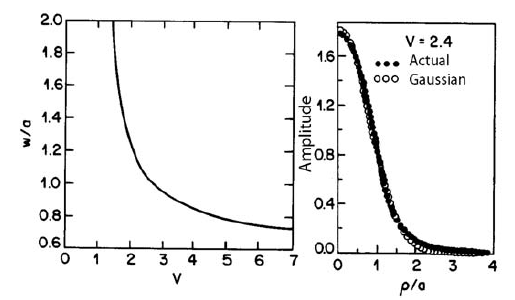
\includegraphics[width=0.6\textwidth]{images/fig2.1.PNG}
                        \caption{Variation of mode-width parameter w with V obtained by fitting the fundamental
                        fiber mode to a Gaussian distribution. Traces on the right show the quality of fit for V = 2.4}
                        \label{fig2.1}
                    \end{figure}
            \end{itemize}
    \subsection{Pulse-Propagation Equation}
        \begin{itemize}
            \item Optical pulses: time width ranging from $\approx10 fs$ to $\approx10 ns$.
            \item The basis of this chapter is \autoref{propagating equation of E with PL and PNL: including laplace symbol}, using \autoref{double crossing laplace relation} and rewrite it here as:
                \begin{equation}
                    \Lap^2\boldsymbol{E} -\frac{1}{c^2}\pdv[2]{\boldsymbol{E}}{t}=\mu_0\pdv[2]{\boldsymbol{P_L}}{t}+\mu_0\pdv[2]{\boldsymbol{P_{NL}}}{t}
                    \label{basis of pulse propagation function: maxwell equation}
                \end{equation}
        \end{itemize}
        
        \subsubsection{Nonlinear Pulse Propagation}
        \begin{itemize}
            \item $\chi$'s Time dependence and Dispersion, as well as their relation:\\
                Usually $\boldsymbol{P}$ is written as
                \begin{subequations}
                    \begin{align}
                        &\boldsymbol{P}_L(\boldsymbol{r}) = \epsilon_0 \chi^{(1)}\cdot\boldsymbol{E}\\
                        &\boldsymbol{P}_{NL}(\boldsymbol{r}) = \epsilon_0 \chi^{(3)} \vdots \boldsymbol{EEE}
                    \end{align}
                    \label{P instantly response to E}
                \end{subequations}
                \autoref{P instantly response to E} is to say that $\boldsymbol{P}$ and $\boldsymbol{E}$ are in simultaneously response:
                \begin{subequations}
                    \begin{align}
                        \chi^{(1)}(t)&=\chi^{(1)}(0)\delta(t),\\
                        \chi^{(3)}(t_1,t_2,t_3)&=\chi^{(3)}(0,0,0)\delta(t_1)\delta(t_2)\delta(t_3).
                    \end{align}
                    \label{no dispersion chi: time domain}
                \end{subequations}
                Also this implies that $\chi$ (1) and (3) don't have dispersion:
                \begin{subequations}
                    \begin{align}
                        \Tilde{\chi}^{(1)}(\omega)&=\Tilde{\chi}^{(1)}(0),\\
                        \Tilde{\chi}^{(3)}(\omega_1,\omega_2,\omega_3)&=\Tilde{\chi}^{(3)}(0,0,0).
                    \end{align}
                    \label{no dispersion chi: freq domain}
                \end{subequations}
                And thus \autoref{P instantly response to E} can be written as:
                \begin{subequations}
                    \begin{align}
                        &\boldsymbol{P}_L(\boldsymbol{r},t)=\epsilon_0\int_{-\infty}^t \chi^{(1)}(t-t^{'})\cdot\boldsymbol{E}(\boldsymbol{r},t^{'})dt^{'}\label{P not instantly response to E, with dispersion: linear part}\\
                        &\boldsymbol{P}_{NL}(\boldsymbol{r},t)=\epsilon_0\int_{-\infty}^t dt_1\int_{-\infty}^t dt_2\int_{-\infty}^t dt_3 \chi^{(3)}(t-t_1,t-t_2,t-t_3)\vdots \boldsymbol{E}(\boldsymbol{r},t_1)\boldsymbol{E}(\boldsymbol{r},t_2)\boldsymbol{E}(\boldsymbol{r},t_3)\label{P not instantly response to E, with dispersion: nonlinear part}
                    \end{align}
                    \label{P not instantly response to E, with dispersion}
                \end{subequations}
                \autoref{P not instantly response to E, with dispersion} is the general expression when \autoref{no dispersion chi: time domain} and \autoref{no dispersion chi: freq domain} don't satisfies. Also to notice that $\chi$ \MakeUppercase{with dispersion means in time domain} $\chi$ \MakeUppercase{has delay in t}. \\The \autoref{P not instantly response to E, with dispersion} is actually a form of convolution. Using the fourier transform properties in convoultion, we can get a form of \autoref{P not instantly response to E, with dispersion} which is more important:
                \begin{subequations}
                \begin{align}
                    &\Tilde{\boldsymbol{P}}_L(\boldsymbol{r},\omega)=\epsilon_0 \chi^{(1)}(\omega)\cdot \boldsymbol{\Tilde{E}}(\boldsymbol{r},\omega)\label{PL not instantly response to E: freq domain}\\
                    &\Tilde{\boldsymbol{P}}_{NL}(\boldsymbol{r},\omega_1+\omega_2+\omega_3)=\epsilon_0 \chi^{(3)}(\omega_1,\omega_2,\omega_3)\vdots \boldsymbol{\Tilde{E}}(\boldsymbol{r},\omega_1)\boldsymbol{\Tilde{E}}(\boldsymbol{r},\omega_2)\boldsymbol{\Tilde{E}}(\boldsymbol{r},\omega_3)\label{PNL not instantly response to EEE: freq domain}
                \end{align}
                \end{subequations}
                It is useful to deeply understand the action of $\chi^{(1)}$ and $\chi^{(3)}$ now. As \autoref{fig: chi1 and chi3 freq domain illustration} shows, although $\chi^{(1)}$ is frequency dependent, it can never produce P response frequency other than input Electric field frequency. In the circumstance here only $\chi^{(3)}$ can produce response other than Electric field frequency. Also interesting to notice that photonic energy conservation:
                \begin{equation}
                    \hbar \omega = \hbar \omega_1 +\hbar \omega_2+\hbar \omega_3
                    \label{photonic energy conservation: four wave expression}
                \end{equation}
                is automatically satisfied in the Fourier transformation from \autoref{P not instantly response to E, with dispersion: nonlinear part} to \autoref{PNL not instantly response to EEE: freq domain}. Practically in future these frequency can either be positive frequency or negative frequency. If two of $\omega_1$, $\omega_2$ and $\omega_3$ are opposite to each other(e.g:$\omega_1+\omega_2=0$), then this is a good model to Raman process. (which is proportional to light intensity)
                \begin{subequations}
                \begin{align}
                    &\boldsymbol{\Tilde{E}}(\omega_1)\boldsymbol{\Tilde{E}}(-\omega_1)=\abs{\boldsymbol{\Tilde{E}}(\omega_1)}^2\\
                    &\Tilde{\boldsymbol{P}}_{NL,Raman}(\omega_3)=\epsilon_0 \chi^{(3)}(\omega_1,\omega_2,\omega_3)\vdots \boldsymbol{\Tilde{E}}(\omega_1)\boldsymbol{\Tilde{E}}(-\omega_1)\boldsymbol{\Tilde{E}}(\omega_3) \propto \abs{\boldsymbol{\Tilde{E}}(\omega_1)}^2
                \end{align}
                    
                \end{subequations}
                
                \begin{figure}[htbp]
                    \centering
                    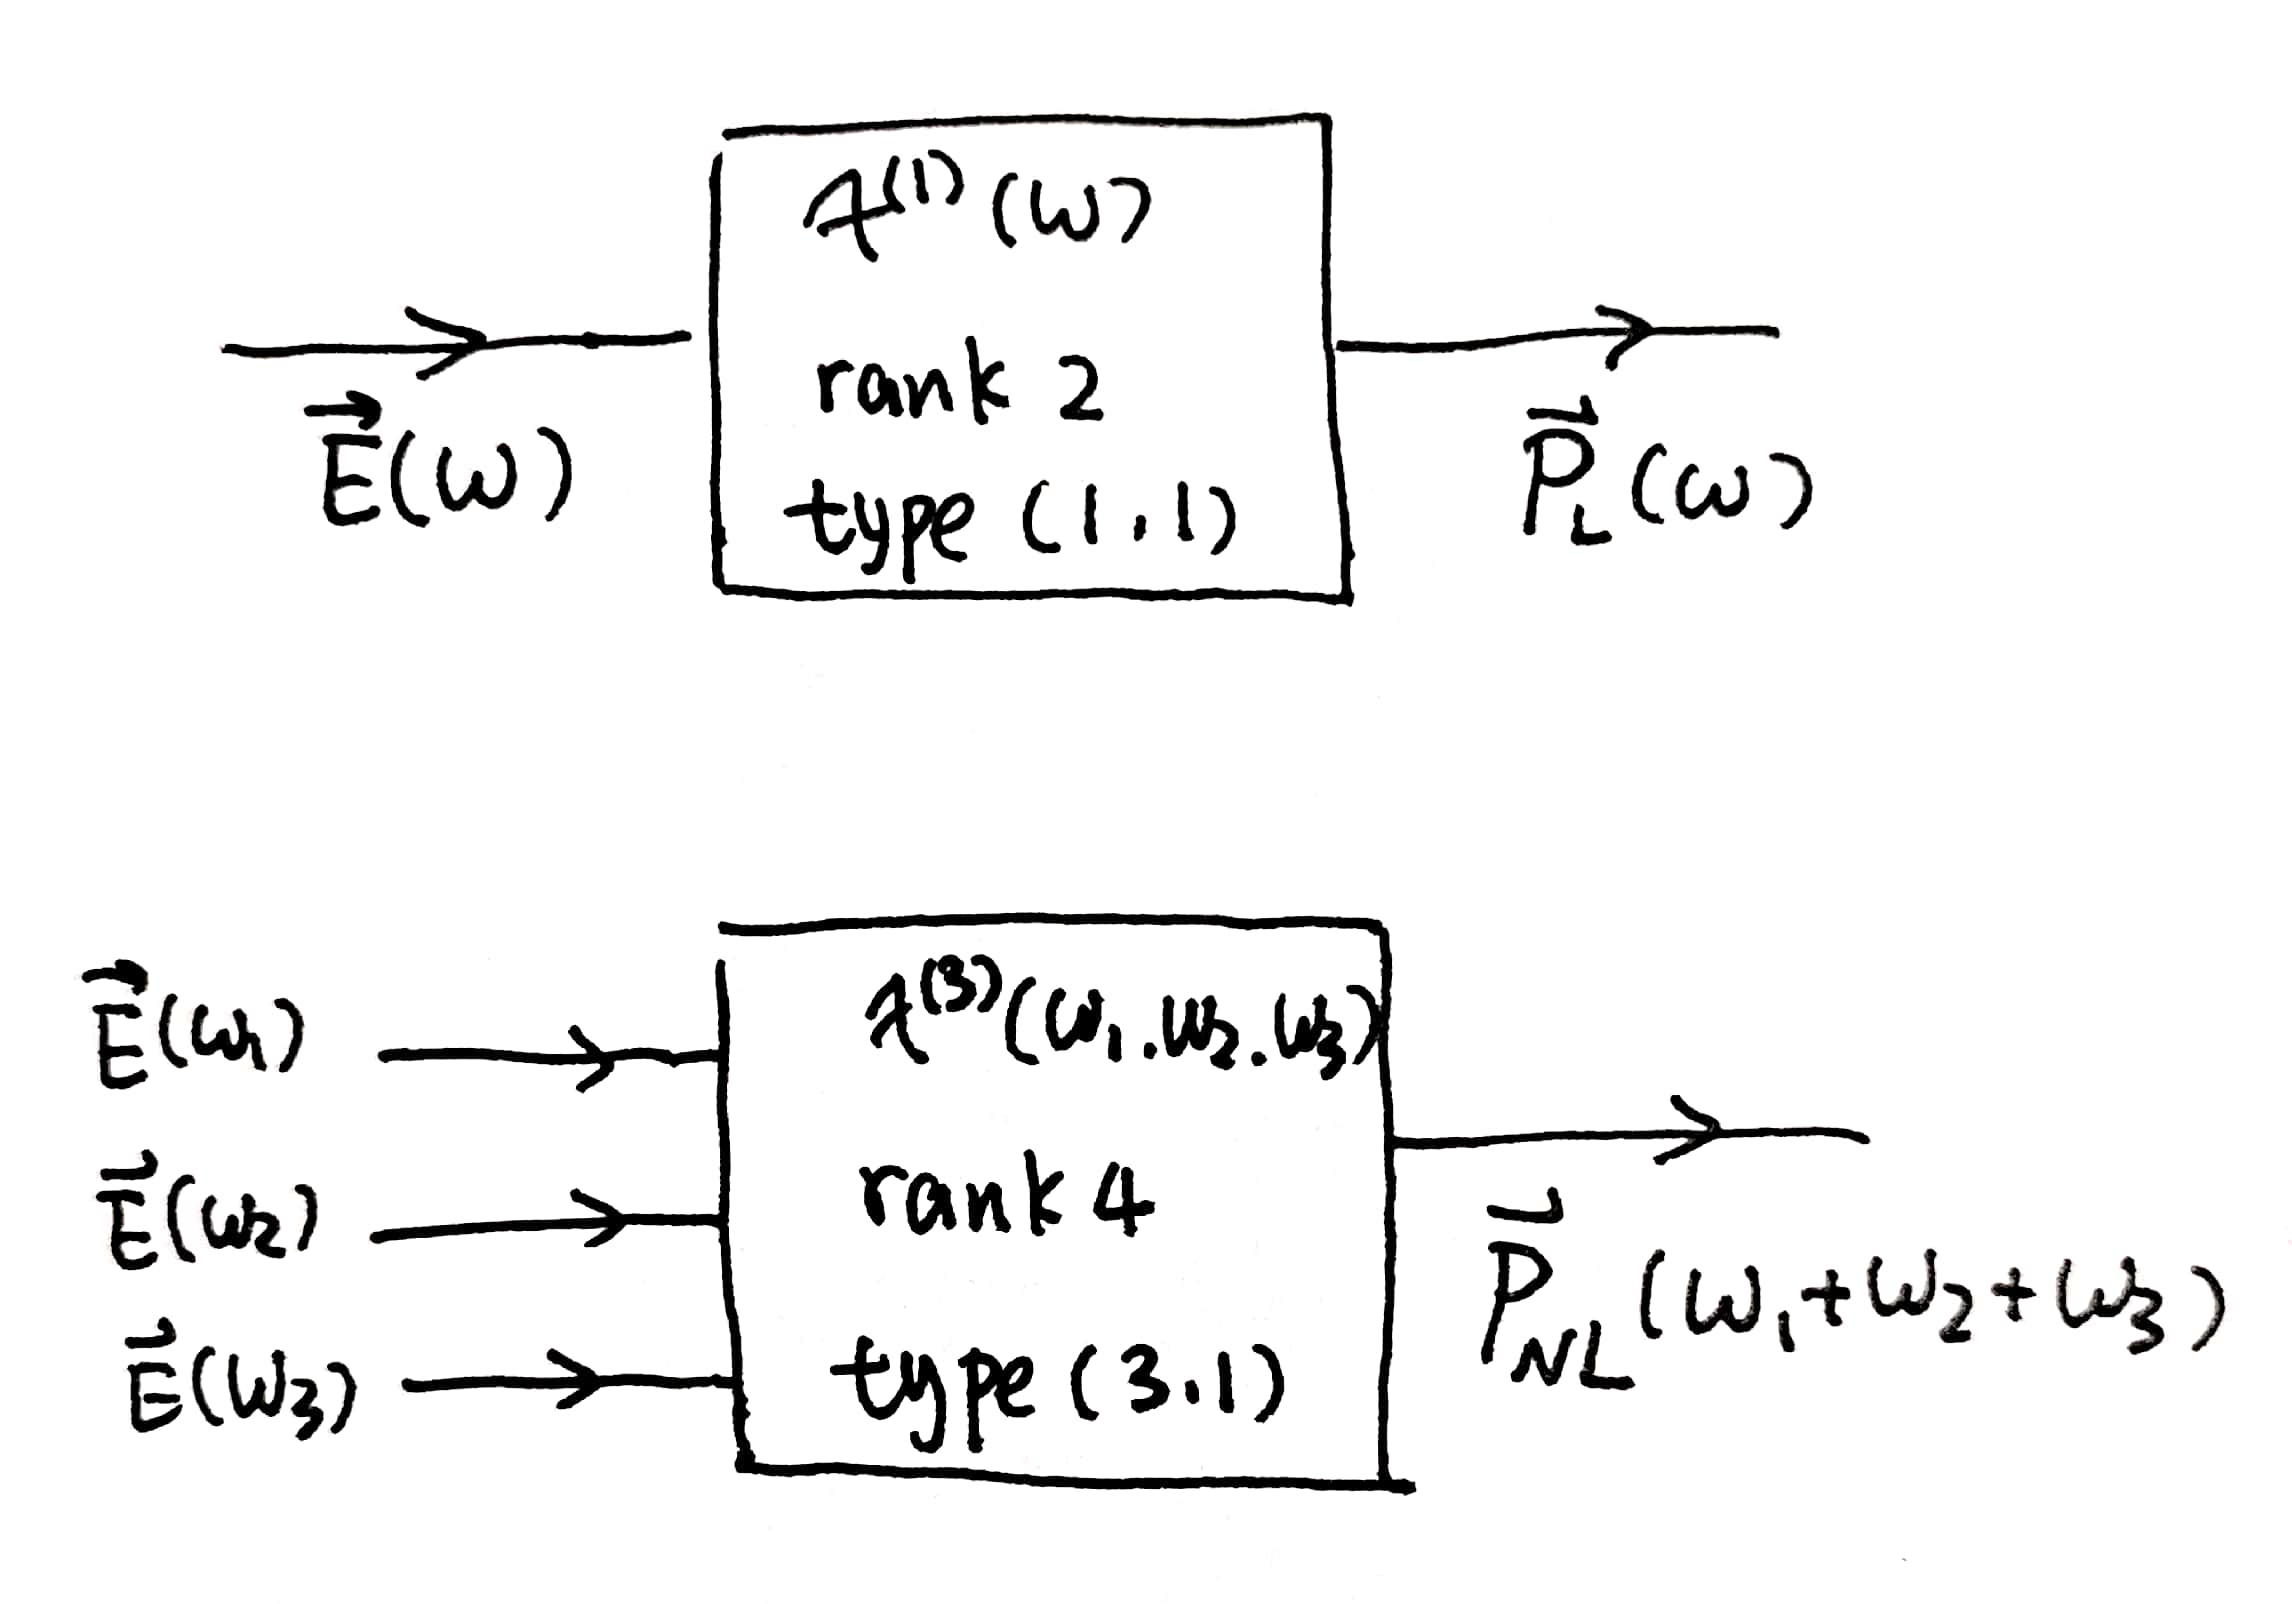
\includegraphics[width=0.6\textwidth]{images/chi1_and_chi3_in_freq_domian.jpg}
                    \caption{Illustration of different functions of $\chi^{(1)}$ and $\chi^{(3)}$. Notice that $\chi^{(1)}$ can never produce P response other than input frequency. Also energy conservation is automatically satisfied in the Fourier transform from \autoref{P not instantly response to E, with dispersion: nonlinear part} to \autoref{PNL not instantly response to EEE: freq domain}.}
                    \label{fig: chi1 and chi3 freq domain illustration}
                \end{figure}
                
                The negative and positive frequency term is actually a phase difference. Classically these two Optical fields:
                \begin{subequations}
                \begin{align}
                    E_1 &= \sin{\omega t}\\
                    E_2 &= -\sin{\omega t} = \sin{-\omega t}
                \end{align}
                \end{subequations}
                
                can be interpreted as having opposite sign of frequency. In classical opinion this can be interpreted as two optical fields cancels each other. In Quantum optics opposite frequency can be interpreted as
                \begin{subequations}
                \begin{align}
                    \hat{a}^\dag &= \hat{E}\exp{-i\omega t}\\
                    \hat{a} &= \hat{E}\exp{i\omega t},
                \end{align}
                \end{subequations}
                which means generation and annihilation of photons.
                
                
            \item Quick evolving term and slow evolving terms separation:\\
                Optical field is assumed to maintain its polarization along the fiber length (which is not the case, but works well). Also optical field is assumed to be quasi-monochromatic, i.e., the pulse spectrum, centered at ω0, is assumed to have a spectral width $\Delta \omega$ such that $\Delta \omega/\omega_0 \ll 1$. Since $\omega_0\approx10^{-15}s^{-1}$, the last assumption is valid for pulses as short as 0.1 ps.
                \begin{subequations}
                \label{fast oscillation separation}
                    \begin{align}
                        \boldsymbol{E}(\boldsymbol{r},t)&=\frac{1}{2}\hat{\boldsymbol{x}}(E(\boldsymbol{r},t)\exp{-i\omega_0 t}+E^{*}(\boldsymbol{r},t)\exp{i\omega_0 t}),\label{fast oscillation separation: E}\\
                        \boldsymbol{P_L}(\boldsymbol{r},t)&=\frac{1}{2}\hat{\boldsymbol{x}}(P_L(\boldsymbol{r},t)\exp{-i\omega_0 t}+P_L^{*}(\boldsymbol{r},t)\exp{i\omega_0 t}),\label{fast oscillation separation: P}\\
                        \boldsymbol{P_{NL}}(\boldsymbol{r},t)&=\frac{1}{2}\hat{\boldsymbol{x}}(P_{NL}(\boldsymbol{r},t)\exp{-i\omega_0 t}+P_{NL}^{*}(\boldsymbol{r},t)\exp{i\omega_0 t}),\label{fast oscillation separation: PNL}\\
                        \boldsymbol{D}(\boldsymbol{r},t)&=\frac{1}{2}\hat{\boldsymbol{x}}(D(\boldsymbol{r},t)\exp{-i\omega_0 t}+D^{*}(\boldsymbol{r},t)\exp{i\omega_0 t}),\label{fast oscillation separation: D}
                    \end{align}
                \end{subequations}
            \item Considerable simplification occurs if the nonlinear response is assumed to be instantaneous,
            \begin{equation}
                \chi^{(3)}(\omega_1,\omega_2,\omega_3)\longrightarrow\chi^{(3)}(\omega)=\chi^{(3)}(\omega,-\omega,\omega)=const,
                \label{chi3 has no dispersion, instantaneous response}
            \end{equation}
            which means $\chi^{(3)}$ has no dispersion. Thus
                \begin{equation}
                    \label{PNL with EEE relation}
                    \boldsymbol{P}_{NL}(\boldsymbol{r}) = \epsilon_0 \chi^{(3)} \vdots \boldsymbol{EEE}
                \end{equation}
                This approximation works well when we neglect the contribution of molecular vibrations to $\chi^{(3)}$ (the Raman effect). In general, both electrons and nuclei respond to the optical field in a nonlinear manner. Nuclei $\approx 60-70fs$. This works well for pulse $>1ps$. Take \autoref{fast oscillation separation: E} and \autoref{fast oscillation separation: PNL} into \autoref{PNL with EEE relation}, we get:
                \begin{equation}
                \begin{split}
                    \boldsymbol{P}_{NL}=& P_{NL,x}\hat{\boldsymbol{x}}+P_{NL,y}\hat{\boldsymbol{y}}+P_{NL,z}\hat{\boldsymbol{z}},\\
                    P_{NL,x}=&\epsilon_0 {{\chi^{(3)}}_x}^{xxx} E_x E_x E_x\\
                    =&\epsilon_0 {{\chi^{(3)}}_x}^{xxx} \frac{1}{8}(E(\boldsymbol{r},t)\exp{-i\omega_0 t}+E^{*}(\boldsymbol{r},t)\exp{i\omega_0 t})^3\\
                    =&\frac{1}{8} \epsilon_0 {{\chi^{(3)}}_x}^{xxx}(3\abs{E(\boldsymbol{r},t)}^2 E(\boldsymbol{r},t)\exp{-i\omega_0 t}+3\abs{E(\boldsymbol{r},t)}^2 E^{*}(\boldsymbol{r},t)\exp{i\omega_0 t}\\
                    &+E^3(\boldsymbol{r},t)\exp{-3i\omega_0 t}+E^{*3}(\boldsymbol{r},t)\exp{3i\omega_0 t})\\
                    =&\frac{1}{2}(P_{NL}(\boldsymbol{r},t)\exp{-i\omega_0 t}+P_{NL}^{*}(\boldsymbol{r},t)\exp{i\omega_0 t}).
                \end{split}
                \end{equation}
                Neglecting freq mismatch terms, we get
                \begin{equation}
                    P_{NL}(\boldsymbol{r},t) = \frac{3}{4}\epsilon_0{{\chi^{(3)}}_x}^{xxx}\abs{E(\boldsymbol{r},t)}^2E(\boldsymbol{r},t).
                \end{equation}
                Thus
                \begin{subequations}
                \begin{align}
                    P_{NL}=&\epsilon_0\epsilon_{NL}E\\
                    \epsilon_{NL}=&\frac{3}{4}{{\chi^{(3)}}_x}^{xxx}\abs{E(\boldsymbol{r},t)}^2\label{Nonlinear epsilon relation with chi3 and E}
                \end{align}
                \end{subequations}
            \item \MakeUppercase{(This bullet is the derivation of }\autoref{Helmholtz equation in frequency domain}, \MakeUppercase{and some simplifications used.} \autoref{Helmholtz equation in frequency domain} is different from \autoref{Propagation E equation in freq domain} because they are respectively slow and fast term equations, in \autoref{fast oscillation separation: E}.)\\Take negative freq terms of \autoref{fast oscillation separation} into \autoref{basis of pulse propagation function: maxwell equation} (notice time derivative to $\exp{-i\omega_0 t}$), we can get (the following omits $(\boldsymbol{r},t)$ in \autoref{fast oscillation separation} for simplicity)
                \begin{equation}
                \begin{split}
                    &\exp{-i\omega_0 t}[\Lap^2 E-\epsilon_0 \mu_0(\pdv[2]{E}{t}-2i\omega_0\pdv{E}{t}-\omega_0^2 E)]\\
                    =&\exp{-i\omega_0 t}\mu_0[\pdv[2]{(P_L+P_{NL})}{t}-2i\omega_0\pdv{(P_L+P_{NL})}{t}-\omega_0^2(P_L+P_{NL})].
                \end{split}
                \label{slow oscillatiing term propagation equation derive in section 2.3.1}
                \end{equation}
                
            % \item \MakeUppercase{(This bullet is the derivation of }\autoref{Helmholtz equation in frequency domain}, \MakeUppercase{and some simplifications used.)}\\Then we try to write slow oscillating term into freq domain:\\
            %     First we do some approximation to \autoref{slow oscillating E term equation in time domain}, which physical meaning are more clear and discussable in freq domain:
            %     We Assume 
           
            %     Then \autoref{slow oscillating E term equation in time domain} is simplified to:
            %     \begin{equation}
            %         \Lap^2E-\frac{1}{c^2}\pdv[2]{E}{t}=\mu_0({{\chi^{(1)}}_x}^x+\epsilon_{NL})\pdv[2]{E}{t}
            %         \label{simplified slow oscillating E term equation in time domain}
            %     \end{equation}
                Here are some relations that we will use to simplify \autoref{slow oscillatiing term propagation equation derive in section 2.3.1}:
                    \SubItem{
                    Fourier transforms:
                    \begin{subequations}
                    \begin{align}
                        &\Tilde{E}(\boldsymbol{r},\omega-\omega_0)=\int_{-\infty}^{\infty}E(\boldsymbol{r},t)\exp{i(\omega-\omega_0)t}dt, \label{fourier transform of slow oscillating term of E}\\
                        &E(\boldsymbol{r},t)=\frac{1}{2\pi}\int_{-\infty}^{\infty}\Tilde{E}(\boldsymbol{r},\omega-\omega_0)\exp{-i(\omega-\omega_0)t}d\omega, \label{inverse fourier transform of slow oscillating term of E}\\
                        &\Tilde{P}_L(\boldsymbol{r},\omega-\omega_0)=\int_{-\infty}^{\infty}P_L(\boldsymbol{r},t)\exp{i(\omega-\omega_0)t}dt, \label{fourier transform of slow oscillating term of PL}\\
                        &P_L(\boldsymbol{r},t)=\frac{1}{2\pi}\int_{-\infty}^{\infty}\Tilde{P}_L(\boldsymbol{r},\omega-\omega_0)\exp{-i(\omega-\omega_0)t}d\omega. \label{inverse fourier transform of slow oscillating term of PL}\\
                        &\Tilde{P}_{NL}(\boldsymbol{r},\omega-\omega_0)=\int_{-\infty}^{\infty}P_{NL}(\boldsymbol{r},t)\exp{i(\omega-\omega_0)t}dt, \label{fourier transform of slow oscillating term of PNL}\\
                        &P_{NL}(\boldsymbol{r},t)=\frac{1}{2\pi}\int_{-\infty}^{\infty}\Tilde{P}_{NL}(\boldsymbol{r},\omega-\omega_0)\exp{-i(\omega-\omega_0)t}d\omega. \label{inverse fourier transform of slow oscillating term of PNL}
                    \end{align}
                    \end{subequations}
                    }
                    \SubItem{
                    And a relation based on neglecting Raman term of nuclei:
                    \begin{equation}
                        %P_L(\boldsymbol{r},t) &= \epsilon_0 {{\chi^{(1)}}_x}^x E(\boldsymbol{r},t)\\
                        P_{NL}(\boldsymbol{r},t)= \epsilon_0 \epsilon_{NL}(\boldsymbol{r},t) E(\boldsymbol{r},t).
                    \label{simplificaiton used in section 2.3.1 to get helmholtz equation}
                    \end{equation}
                    Reminder: 
                    \begin{itemize}
                        \item $\epsilon_{NL}$ in \autoref{simplificaiton used in section 2.3.1 to get helmholtz equation} is actually time dependent based on \autoref{Nonlinear epsilon relation with chi3 and E}. However ${{\chi^{(3)}}_x}^{xxx}$ is NOT time dependent here based on the simplification from \autoref{P not instantly response to E, with dispersion: nonlinear part} to \autoref{PNL with EEE relation}.
                        \item This simplification only neglected the Raman term from nuclei. The Raman term from electrons are also neglected in \autoref{Helmholtz equation in frequency domain}, HOWEVER NOT YET. 
                    \end{itemize}
                    }
                    
                    
                Now come back to simplify \autoref{slow oscillatiing term propagation equation derive in section 2.3.1}. First put \autoref{simplificaiton used in section 2.3.1 to get helmholtz equation} into \autoref{slow oscillatiing term propagation equation derive in section 2.3.1}, we get
                \begin{equation}
                \begin{split}
                    &[\Lap^2 E-\epsilon_0 \mu_0(\pdv[2]{E}{t}-2i\omega_0\pdv{E}{t}-\omega_0^2 E)]\\
                    =&\mu_0[\pdv[2]{(P_L+\epsilon_0 \epsilon_{NL} E)}{t}-2i\omega_0\pdv{(P_L+\epsilon_0 \epsilon_{NL} E)}{t}-\omega_0^2(P_L+\epsilon_0 \epsilon_{NL} E)].
                \end{split}
                \label{slow oscillatiing term propagation equation derive in section 2.3.1-part 2}
                \end{equation}
                Now neglect time derivative terms of $\epsilon_{NL}$:
                \begin{equation}
                \begin{split}
                    &[\Lap^2 E-\epsilon_0 \mu_0(\pdv[2]{E}{t}-2i\omega_0\pdv{E}{t}-\omega_0^2 E)]\\
                    =&\mu_0[\pdv[2]{P_L}{t}-2i\omega_0\pdv{P_L}{t}-\omega_0^2P_L]+\mu_0\epsilon_0\epsilon_{NL}[\pdv[2]{E}{t}-2i\omega_0\pdv{E}{t}-\omega_0^2 E].
                \end{split}
                \label{slow oscillatiing term propagation equation derive in section 2.3.1-part 3}
                \end{equation}
                
                
                Then put \autoref{inverse fourier transform of slow oscillating term of E} and \autoref{inverse fourier transform of slow oscillating term of PL} into \autoref{slow oscillatiing term propagation equation derive in section 2.3.1-part 3}, \\
                Note in detail that some terms are cancelled:
                \begin{equation}
                \begin{split}
                    &\pdv[2]{E}{t}-2i\omega_0\pdv{E}{t}-\omega_0^2 E\\
                    =&\frac{1}{2\pi}\int_{-\infty}^{\infty}\Tilde{E}(\boldsymbol{r},\omega-\omega_0)[(-i(\omega-\omega_0))^2-2i\omega_0(-i(\omega-\omega_0))-\omega_0^2]\exp{-i(\omega-\omega_0)t}d\omega\\
                    =&\frac{1}{2\pi}\int_{-\infty}^{\infty}\Tilde{E}(\boldsymbol{r},\omega-\omega_0)[-\omega^2]\exp{-i(\omega-\omega_0)t}d\omega
                \end{split}
                \label{slow oscillatiing term propagation equation derive in section 2.3.1-part 4}
                \end{equation}
                we get
                \begin{equation}
                    \Lap^2\Tilde{E}+k^2\Tilde{E}=-\mu_0 \omega^2 \Tilde{P}_L- \epsilon_{NL}k^2\Tilde{E},
                    \label{slow oscillatiing term propagation equation derive in section 2.3.1-part 5}
                \end{equation}
                where
                \begin{equation}
                    k=\frac{\omega}{c}.
                \end{equation}
                Then put \autoref{PL not instantly response to E: freq domain} into \autoref{slow oscillatiing term propagation equation derive in section 2.3.1-part 5}, (These two equations are both in freq domain, and \autoref{PL not instantly response to E: freq domain} are actually precise without any assumption of instant response)\\
                We get Helmholtz equation
                \begin{equation}
                    \Lap^2\Tilde{E}+\epsilon(\omega)k^2\Tilde{E}=0,
                    \label{Helmholtz equation in frequency domain}
                \end{equation}
                where
                \begin{equation}
                    \epsilon(\omega)=1+{{\chi^{(1)}}_x}^x(\omega)+\epsilon_{NL}
                    \label{epsilon omega relation to chi1 and epsilon nl}
                \end{equation}
                
                
                Now we need to discuss the physics meaning from \autoref{slow oscillatiing term propagation equation derive in section 2.3.1-part 2} to \autoref{slow oscillatiing term propagation equation derive in section 2.3.1-part 3}. From \autoref{slow oscillatiing term propagation equation derive in section 2.3.1-part 2} to \autoref{slow oscillatiing term propagation equation derive in section 2.3.1-part 3}, we actually assumed the time derivative of $\epsilon_{NL}$ (\autoref{Nonlinear epsilon relation with chi3 and E}) is small. From the contents and conclusions of \autoref{P not instantly response to E, with dispersion}, we know this approximation actually has some impact in frequency domain. That's why in \autoref{epsilon omega relation to chi1 and epsilon nl} $\epsilon_{NL}$ term was not indicated as $\epsilon_{NL}(\omega)$.
                %     \SubItem{The impact of simplificating ${{\chi^{(1)}}_x}^x$ from \autoref{P not instantly response to E, with dispersion: linear part} is kind of complicated.
                %         \begin{equation}
                %         \begin{split}
                %             \pdv[2]{P_L}{t}=&\epsilon_0\pdv[2]{\int_{-\infty}^t \chi^{(1)}(t-t^{'})\cdot\boldsymbol{E}(\boldsymbol{r},t^{'})dt^{'}}{t}\\
                %             =&???(intentionally Left Blank)\\
                %             =&{omitted Terms}+\epsilon_0{{\chi^{(1)}}_x}^x \pdv[2]{E(\boldsymbol{r},t)}{t}.
                %         \end{split}
                %         \end{equation}
                %     }
                    \SubItem{The impact of $\epsilon_{NL}$ can be derived from \autoref{Nonlinear epsilon relation with chi3 and E}. To write out terms we neglected from \autoref{slow oscillatiing term propagation equation derive in section 2.3.1-part 2} to \autoref{slow oscillatiing term propagation equation derive in section 2.3.1-part 3}, we write this derive in detail:
                        \begin{equation}
                        \begin{split}
                            \pdv[2]{P_{NL}}{t}=&\pdv[2]{\epsilon_0\epsilon_{NL}(\boldsymbol{r},t)E(\boldsymbol{r},t)}{t}\\
                            =&\epsilon_0[\epsilon_{NL}\pdv[2]{E(\boldsymbol{r},t)}{t}+2\pdv{\epsilon_{NL}(\boldsymbol{r},t)}{t}\pdv{E(\boldsymbol{r},t)}{t}+E(\boldsymbol{r},t)\pdv[2]{\epsilon_{NL}(\boldsymbol{r},t)}{t}]\\
                            =&\epsilon_0[\epsilon_{NL}\pdv[2]{E}{t}+\frac{3}{2}{{\chi^{(3)}}_x}^{xxx}\pdv{\abs{E}^2}{t}\pdv{E}{t}+E\frac{3}{4}{{\chi^{(3)}}_x}^{xxx}\pdv[2]{\abs{E}^2}{t}].
                        \end{split}
                        \label{electron raman term due to epsilon NL time dependance}
                        \end{equation}
                        And the terms we neglected is the second and third term in \autoref{electron raman term due to epsilon NL time dependance}:
                        \begin{equation}
                            \frac{3}{2}{{\chi^{(3)}}_x}^{xxx}\pdv{\abs{E}^2}{t}\pdv{E}{t}+E\frac{3}{4}{{\chi^{(3)}}_x}^{xxx}\pdv[2]{\abs{E}^2}{t}.
                        \end{equation}
                        These are actually electron Raman terms. Refer to the reminder below \autoref{simplificaiton used in section 2.3.1 to get helmholtz equation}, we actually included no Raman at all in \autoref{Helmholtz equation in frequency domain}. HOWEVER the electron and nuclei Raman terms are neglected at different steps.\\ \\ Later we will discuss more about Raman term. The reason why electron Raman term is not important is based on the assumption that:
                        \begin{equation}
                            \pdv[2]{E}{t} \ll \omega_0 \pdv{E}{t}.
                            \label{slow oscillating term second order derivative is much smaller than first order}
                        \end{equation}
                        Thus second order derivative is much smaller than first order. \\
                        This is consistent with \autoref{fast oscillation separation: E}, in which we already assumed E                        is slow oscillating term and $\Delta \omega \ll \omega_0$. We will come back to this assumption when we discuss Raman term later.
                    }
            \item \MakeUppercase{This bullet is to clarify some common misconstrue of} \autoref{slow oscillatiing term propagation equation derive in section 2.3.1}.\\ The slow oscillating term and quick oscillating term in \autoref{fast oscillation separation: E} satisfy different equations.
            Only if we assume (Here D is the same in \autoref{fast oscillation separation: D})
                \begin{subequations}
                \begin{align*}
                    &2i\omega_0\pdv{D}{t}+\omega_0^2 D=0,\\
                    where: & D = \epsilon_0 E +P_L+P_{NL},
                \end{align*}
                \label{D approximation in section 2.3.1}
                \end{subequations}
                \MakeUppercase{which is apparently wrong,} can we get propagation equation of slow oscillating term in \autoref{fast oscillation separation} satisfies a similar form of fast oscillating term.\\ By taking the above D relation into \autoref{slow oscillatiing term propagation equation derive in section 2.3.1}, we get slow oscillating term equation which is similar to fast term:
                \begin{equation*}
                    \Lap^2E-\frac{1}{c^2}\pdv[2]{E}{t}=\mu_0\pdv[2]{(P_L+P_{NL})}{t}.
                \end{equation*}
                \MakeUppercase{However this is also wrong!}
            \item Similar to \autoref{relation between epsilon, n and alpha}, here both $n$ and $\alpha$ is intensity dependent because of $\epsilon_{NL}$ in \autoref{epsilon omega relation to chi1 and epsilon nl}. It is customary to introduce
            \begin{subequations}
                \begin{align}
                    \Tilde{n}&=n+\Bar{n}_2\abs{E}^2,\label{tilde n and n n2 relation}\\
                    \Tilde{\alpha}&=\alpha+\alpha_2\abs{E}^2\label{tilde alpha and alpha alpha2 relation}.
                \end{align}
            \end{subequations}
            And \autoref{relation between epsilon, n and alpha} becomes
            \begin{equation}
                \epsilon(\omega, \abs{E}^2) = (\Tilde{n}+\frac{i\Tilde{\alpha}}{2k})^2.
                \label{relation between tilde epsilon, tilde n and tilde alpha}
            \end{equation}
            The nonlinear-index coefficient $\Bar{n}_2$ and the two-photon absorption coefficient $\alpha_2$ are given by
            \begin{subequations}
                \begin{align}
                    \Bar{n}_2&=\frac{3}{8n}\Re{\chiThree},\label{nonlinear-index coefficient bar n2 relation to chi3}\\
                    \alpha_2&=\frac{3\omega_0}{4nc}\Im{\chiThree} \label{two-photon absorption coefficient alpha2 relation to chi3}.
                \end{align}
            \end{subequations}
            
            \item Solving \autoref{Helmholtz equation in frequency domain}:\\
            variable seperation:
            \begin{equation}
                \Tilde{E}(\boldsymbol{r},\omega-\omega_0)=F(x,y)\Tilde{A}(z,\omega-\omega_0)\exp{i\beta_0 z}.
                \label{tilde E seperate to F, A and exp(ibeta z)}
            \end{equation}
            $F(x,y)$ has the unit of length, $\Tilde{A}(z,\omega-\omega_0)$ has the umit of $V/m$. Notice $\Tilde{A}(z,\omega-\omega_0)$ is slow varying function of z. 
            \begin{subequations}
            \begin{align}
                \pdv[2]{F}{x}+\pdv[2]{F}{x}+[\epsilon(\omega)k^2-\Tilde{\beta}^2]F &= 0 \label{dynamic equation of F: mode on cross section}\\
                2i\beta\pdv{\Tilde{A}}{z}+(\Tilde{\beta}^2-\beta_0^2)\Tilde{A}&=0 \label{dynamic equation of A, freq domain: slow oscillating term}.
            \end{align}
            \end{subequations}
            Notice \autoref{dynamic equation of A, freq domain: slow oscillating term} neglected second derivative $\pdv[2]{\Tilde{A}}{z}$, as $\Tilde{A}$ is slow varying term.\\
            \SubItem{\textbf{Step 1: Separate Orders}\\
                $\epsilon(\omega)$ in \autoref{dynamic equation of F: mode on cross section} is the same as \autoref{epsilon omega relation to chi1 and epsilon nl}, which can be approximated by (use \autoref{tilde n and n n2 relation} and \autoref{relation between tilde epsilon, tilde n and tilde alpha}):
                \begin{equation}
                \begin{split}
                    \epsilon(\omega, \abs{E}^2) &= (\Tilde{n}+\frac{i\Tilde{\alpha}}{2k_0})^2\\
                    &=(n(\omega)+\Bar{n}_2\abs{E}^2+\frac{i\Tilde{\alpha}}{2k_0})^2\\
                    &=(n(\omega)+\Delta n)^2 \approx n^2+2n\Delta n,
                \end{split}
                \end{equation}
                where (note n is not intensity dependent)
                \begin{equation}
                    \Delta n(\omega, \abs{E}^2) = \Bar{n}_2\abs{E}^2+\frac{i\Tilde{\alpha}(\omega, \abs{E}^2)}{2k_0}.
                    \label{Delta n relation with abs E and alpha}
                \end{equation}
            }
            \SubItem{\textbf{Step 2: First order solution}\\
                Treat $\Delta n$ as a perturbation. First replace $\epsilon$ as $n^2$, get $F(x,y)$ from \autoref{dynamic equation of F: mode on cross section} and corresponding wave number $\beta(\omega)$. This solution is useful to expand around the carrier freq $\omega_0$ as:
                \begin{equation}
                    \beta(\omega) = \beta_0 + (\omega-\omega_0)\beta_1 + \frac{1}{2}(\omega-\omega_0)^2\beta_2 + \frac{1}{6}(\omega-\omega_0)^3\beta_3 + \dots,
                    \label{beta omega expands around omega 0}
                \end{equation}
                where
                \begin{equation}
                    \beta_m = (\dv[m]{\beta}{\omega})_{\omega=\omega_0}     (m=1,2,\dots).
                    \label{beta m expression as beta derivative}
                \end{equation}
                (Refer \autoref{group velocity and group index} and \autoref{beta2 definition} to recall their physical relation to group velocity and GVD.)\\
                And it is notable that $\beta(\omega_0)=\beta_0$ which is the same $\beta_0$ in \autoref{dynamic equation of A, freq domain: slow oscillating term}. Although this process is precisely analytical, the simple intuitive physical meaning of $\beta$ is wave number also works. The approximation:
                \begin{equation}
                    \beta(\omega) \approx n(\omega)\frac{\omega}{c}
                    \label{beta omega relation approx to n omega / c}
                \end{equation}
                may not be precise, but still correct.(Refer \autoref{propagation constant expansion} actually contains approximation.)
            }
            \SubItem{\textbf{Step 3: High order correction to wave number}\\
                Then include $\Delta n$. \MakeUppercase{In first order perturbation theory, } $\Delta n$ \MakeUppercase{does not affect }$F(x,y)$, \MakeUppercase{ however can affect wave number as:}
                \begin{equation}
                    \Tilde{\beta}(\omega) = \beta(\omega) + \Delta \beta(\omega),
                    \label{tilde beta and delta beta relation}
                \end{equation}
                where
                \begin{equation}
                    \Delta \beta(\omega) = \frac{\omega^2 n(\omega)}{c^2 \beta(\omega)} \frac{\iint _{-\infty}^\infty \Delta n(\omega) \abs{F(x,y)}^2 \mathrm{dxdy}}{\iint_{-\infty}^\infty \abs{F(x,y)}^2 \mathrm{dxdy}}.
                    \label{delta beta intergral relation with F(x,y)}
                \end{equation}
                Similiary expand $\Delta \beta$ around $\omega_0$, we get
                \begin{equation}
                    \Delta \beta(\omega) = \Delta \beta_0 + (\omega-\omega_0)\Delta \beta_1 + \frac{1}{2}(\omega-\omega_0)^2\Delta \beta_2 + \frac{1}{6}(\omega-\omega_0)^3\Delta \beta_3 + \dots,
                    \label{Delta beta omega expands around omega 0}
                \end{equation}
                where
                \begin{equation}
                    \Delta \beta_m = (\dv[m]{\Delta \beta}{\omega})_{\omega=\omega_0}     (m=1,2,\dots).
                    \label{Delta beta m expression as Delta beta derivative}
                \end{equation}
            }
            
            Recall that from \autoref{fast oscillation separation: E} and \autoref{tilde E seperate to F, A and exp(ibeta z)}, electric field can be written as:
            \begin{equation}
                \boldsymbol{E}(\boldsymbol{r},t)=\frac{1}{2}\boldsymbol{\hat{x}}[F(x,y)A(z,t)\exp{i(\beta_0 z-\omega_0 t)}+c.c].
            \end{equation}
            
            \SubItem{\textbf{Step 4: Get Pulse Propagation Equation}\\
            Neglect high order small magnitude, approximate $\Tilde{\beta}^2-\beta_0^2$ by $2\beta_0(\Tilde{\beta}-\beta_0)$, \autoref{dynamic equation of A, freq domain: slow oscillating term} can be written as:
            \begin{equation}
                \pdv{\Tilde{A}}{z}=i[\beta(\omega)+\Delta \beta(\omega)-\beta_0]\Tilde{A}.
            \end{equation}
            Take Fourier transform as
            \begin{equation}
                A(z,t)=\frac{1}{2\pi}\int_{-\infty}^\infty\Tilde{A}(z,\omega-\omega_0)\exp{-i(\omega-\omega_0)t}d\omega.
                \label{Fourier transform from tilde A to A}
            \end{equation}
            The resulting equation of $A(z,t)$ becomes
            \begin{equation}
                \pdv{A}{z}+\beta_1\pdv{A}{t}+\frac{i\beta_2}{2}\pdv[2]{A}{t}=i\Delta \beta_0 A,
                \label{dynamic equation of A, time domain, alpha not explicit yet: slow oscillating term}
            \end{equation}
            where $\Delta \beta_0$ can be obtained by take $\omega=\omega_0$ at \autoref{delta beta intergral relation with F(x,y)}:
                \begin{equation}
                \begin{split}
                    &\Delta \beta_0 = \Delta \beta(\omega_0)\\
                    =& \frac{\omega_0^2 n(\omega_0)}{c^2 \beta(\omega_0)} \frac{\iint_{-\infty}^\infty \Delta n(\omega_0) \abs{F(x,y)}^2 \mathrm{dxdy}}{\iint_{-\infty}^\infty \abs{F(x,y)}^2 \mathrm{dxdy}} \mbox{ (Take $\omega_0$ into \autoref{delta beta intergral relation with F(x,y)})}\\
                    =&\frac{\omega_0}{c} \frac{\iint_{-\infty}^\infty \Delta n(\omega_0) \abs{F(x,y)}^2 \mathrm{dxdy}}{\iint_{-\infty}^\infty \abs{F(x,y)}^2 \mathrm{dxdy}} \mbox{ (Used \autoref{beta omega relation approx to n omega / c}: $\beta(\omega_0)\approx n(\omega_0)\omega_0/c$)}\\
                    =&\frac{\omega_0}{c} \frac{\iint_{-\infty}^\infty [\Bar{n}_2\abs{E}^2+\frac{i\Tilde{\alpha}}{2k_0}] \times \abs{F(x,y)}^2 \mathrm{dxdy}}{\iint_{-\infty}^\infty \abs{F(x,y)}^2 \mathrm{dxdy}} \mbox{ (Used \autoref{Delta n relation with abs E and alpha})}\\
                    =&\frac{\omega_0}{c} \frac{\iint_{-\infty}^\infty [\Bar{n}_2\abs{F(x,y)A(z,t)}^2+\frac{i\Tilde{\alpha}}{2k_0}] \times \abs{F(x,y)}^2 \mathrm{dxdy}}{\iint_{-\infty}^\infty \abs{F(x,y)}^2 \mathrm{dxdy}} \mbox{ (Used \autoref{tilde E seperate to F, A and exp(ibeta z)})}\\
                    =&\frac{i\alpha}{2}+\frac{\omega_0\abs{A(z,t)}^2}{c} \frac{\iint_{-\infty}^\infty \Bar{n}_2 \abs{F(x,y)}^4 \mathrm{dxdy}}{\iint_{-\infty}^\infty \abs{F(x,y)}^2 \mathrm{dxdy}} \mbox{ (Neglected $\alpha_2\abs{E}^2$ in \autoref{tilde alpha and alpha alpha2 relation})}\\
                    =&\frac{i\alpha}{2}+\frac{\omega_0\Bar{n}_2}{c}\abs{A}^2 \frac{\iint_{-\infty}^\infty  \abs{F(x,y)}^4 \mathrm{dxdy}}{\iint_{-\infty}^\infty \abs{F(x,y)}^2 \mathrm{dxdy}} \mbox{ (Neglected $\Bar{n}_2$ difference between core and cladding)}\\
                    =&\frac{i\alpha}{2}+\gamma(\omega_0)\abs{A}^2,
                    \label{Delta beta omega 0 expression as F(x,y) intergral}                    
                \end{split}
                \end{equation}
                and
                \begin{equation}
                    \gamma(\omega_0) = \frac{\omega_0\Bar{n}_2}{c} \frac{\iint_{-\infty}^\infty  \abs{F(x,y)}^4 \mathrm{dxdy}}{\iint_{-\infty}^\infty \abs{F(x,y)}^2 \mathrm{dxdy}}.
                    \label{gamma omega0 relation in intergral of F(x,y) form}
                \end{equation}
                Finally \autoref{dynamic equation of A, time domain, alpha not explicit yet: slow oscillating term} becomes:
                \begin{equation}
                    \pdv{A}{z}+\beta_1\pdv{A}{t}+\frac{i\beta_2}{2}\pdv[2]{A}{t}+\frac{\alpha}{2}A=i\gamma(\omega_0) \abs{A}^2 A.
                    \label{dynamic equation of A, time domain, alpha explicit: slow oscillating term}
                \end{equation}
            }
            
            \SubItem{\textbf{Step 5: Re-organize units}\\
            The $A(z,t)$ in \autoref{dynamic equation of A, time domain, alpha explicit: slow oscillating term} has the unit of $V/m$ (Refer to \autoref{tilde E seperate to F, A and exp(ibeta z)}). For practical reason, it is common to normalize A such that $\abs{A}^2$ represents optical power. Re normalization as:
            \begin{equation}
                \abs{A^\prime}^2=\frac{1}{2}\epsilon_0 n c \mathcal{A}_m\abs{A}^2,
                \label{renormalization of A to A prime}
            \end{equation}
            where
            \begin{equation}
                \mathcal{A}_m = \iint_{-\infty}^\infty \abs{F(x,y)}^2 \mathrm{dxdy}
                \label{Am definition of intergral}
            \end{equation}
            has the units of $m^4$.\\
            Then it is easy to notice that $\abs{A^\prime}^2$ in \autoref{renormalization of A to A prime} satisfies the same equation as \autoref{dynamic equation of A, time domain, alpha explicit: slow oscillating term}, with the substitution:
            \begin{equation}
                \gamma^\prime(\omega_0)= \frac{\gamma(\omega_0)}{\frac{1}{2}\epsilon_0 n c \mathcal{A}_m}.
                \label{gamma prime defination of gamma and Am}
            \end{equation}
            Thus redefine \autoref{dynamic equation of A, time domain, alpha explicit: slow oscillating term} as the following:
                \begin{equation}
                    \pdv{A^\prime}{z}+\beta_1\pdv{A^\prime}{t}+\frac{i\beta_2}{2}\pdv[2]{A^\prime}{t}+\frac{\alpha}{2}A^\prime=i\gamma^\prime(\omega_0) \abs{A^\prime}^2 A^\prime
                    \label{pulse propagation function without Ramann}
                \end{equation}
                , where
                \begin{equation}
                \begin{split}
                    \gamma^\prime(\omega_0)&= \frac{\gamma(\omega_0)}{\frac{1}{2}\epsilon_0 n c \iint_{-\infty}^\infty \abs{F(x,y)}^2 \mathrm{dxdy}} \mbox{ (Combine \autoref{Am definition of intergral} and \autoref{gamma prime defination of gamma and Am})}\\
                    &=\frac{\omega_0\Bar{n}_2}{c} \frac{\iint_{-\infty}^\infty  \abs{F(x,y)}^4 \mathrm{dxdy}}{\iint_{-\infty}^\infty \abs{F(x,y)}^2 \mathrm{dxdy}} \frac{1}{\frac{1}{2}\epsilon_0 n c \iint_{-\infty}^\infty \abs{F(x,y)}^2 \mathrm{dxdy}} \mbox{ (Used \autoref{gamma omega0 relation in intergral of F(x,y) form})}\\
                    &=\frac{\omega_0}{c}\frac{2\Bar{n}_2}{\epsilon_0 n c} \frac{\iint_{-\infty}^\infty  \abs{F(x,y)}^4 \mathrm{dxdy}}{(\iint_{-\infty}^\infty \abs{F(x,y)}^2 \mathrm{dxdy})^2}\\
                    &=\frac{\omega_0}{c}n_2\frac{1}{A_{eff}}.
                    \label{gamma prime relation with F(x,y) as intergral form}
                \end{split}
                \end{equation}
                And
                \begin{subequations}
                \begin{align}
                    n_2 &= \frac{2\Bar{n}_2}{\epsilon_0 n c},\label{n2 definition, nonlinear Kerr parameter with units of m2/W}\\
                    A_{eff} &= \frac{(\iint_{-\infty}^\infty \abs{F(x,y)}^2 \mathrm{dxdy})^2}{\iint_{-\infty}^\infty  \abs{F(x,y)}^4 \mathrm{dxdy}}.\label{effective mode area Aeff definition}
                \end{align}
                \end{subequations}
                Usually $^\prime$ is omitted in the following text refer to quantities with prime.  $\gamma$ and $A$ in \autoref{dynamic equation of A, time domain, alpha explicit: slow oscillating term} will not be used later.\\
                It is useful to take special notice on the units of $n_2$ and $A_{eff}$. $n_2$ has the unit of $m^2/W$, inverse of optical intensity's unit, which has been discussed as $n_2^I$ at \autoref{n2 and n2I relation}. Typical value of $n_2$ is $\approx 2.6\times10^{-20} m^2/W$.\\
                Unlike \autoref{Am definition of intergral} has a strange unit, \autoref{effective mode area Aeff definition} has a reasonable unit of area, it is so called \MakeUppercase{effective mode area}. To estimate effective mode area, we can use
                \begin{equation}
                    A_{eff} = \pi w^2
                \end{equation}
                , where $w$ can be obtained from V factor(\autoref{V parameter}) or mode approximation(\autoref{fig2.1}).
            }
            \item Highly nonlinear fibers: Typically, $A_{eff}$ varies around $1-100\mu m^2$, depending on fiber design. In order to have a high non-linear effect(high $\gamma\prime$ in \autoref{gamma prime relation with F(x,y) as intergral form}), specially designed small $A_{eff}$ is required. $\gamma\prime$ values in range $1-100W^{-1}/km$.
            \item Finally, it must be highlighted that \autoref{pulse propagation function without Ramann} can only be used for pulses not too short(>1ps). Otherwise some approximations used in the derivation are questionable.
        \end{itemize}
        
    \subsubsection{Higher-Order Nonlinear Effects}
        \autoref{pulse propagation function without Ramann} doesn't include effects of stimulated inelastic scattering such as SRS and SBS. If peak power of the incident pulse is above a threshold level, SRS and SBS can transfer energy to a new pulse at a different wavelength, which may propagate in the same or the opposite direction.\\
        In the case of a delayed Raman response governed by $R(t)$, R(t) is the possibility that $P_{NL}$ gives response at time t. Thus R(t) should satisfy following properties:
        \begin{subequations}
        \begin{align}
            &\int_{-\infty}^\infty R(t)dt=1,\\
            &T_R = <T> = \int_{-\infty}^\infty tR(t)dt,
        \end{align}
        \end{subequations}
        $T_R$ is called \MakeUppercase{the first moment of the Raman response function}. Raman response is an \MakeUppercase{intensity based response}, thus Nonlinear response function will have the following form:
        \begin{equation}
            \chi^{(3)}(t-t_1,t-t_2,t-t_3)=\chi^{(3)}R(t-t_1)\delta(t_1-t_2)\delta(t-t_3),
        \end{equation}
        which can be interpreted as $P_{NL}$ is taking time $t-t_1$(same as $t-t_2$, due to $\delta(t_1-t_2)$ term) to response to field $E_1$(same $E_2$, thus $\abs{E_1}^2$, same $\abs{E_2}^2$), but instantaneously response to $E_3$.(due to $\delta(t-t_3)$ term)\\
        Nonlinear response function can also be written in a symmetrized form:
        \begin{equation}
            \chi^{(3)}(t_1,t_2,t_3)=\chi^{(3)}[R(t_1)\delta(t_2)\delta(t_3-t_1)+\delta(t_1-t_2)R(t_2)\delta(t_3)+\delta(t_1)\delta(t_2-t_3)R(t_3)],
        \end{equation}
        which can be interpreted as first term has delayed response to $E_1$ and $E_3$, but instantaneously response to $E_2$, other terms argues similarly.
        
    \subsubsection{Raman Response Function}
    
    \subsection{Numerical Methods}
            
\newpage
\section{Group-Velocity Dispersion}

\subsection{Different Propagation Regimes}








% \subsubsection{effective red and blue detune}


% \section{Coupling mode equation}


% \section{Soliton generation}
% \subsection{modulation instability}


% \subsection{Turing pattern}
% \subsection{Bright cavity soliton}
% \subsection{Bright soliton molecules}
% \subsection{Breathing solitons}


% \section{Induction Proofs}
% \subsection{Ordinary Induction}
% \begin{exercise} Prove, for all natural numbers $n$, that 
% \begin{equation} \sum_{k=0}^n k = 1 + 2 + 3 + \cdots + n = \dfrac{n(n+1)}{2}
% \label{eq:Pn}\end{equation}
% \end{exercise}

% \begin{proof}
% We prove this by induction on $n\in\N$.  In the base case, $n=0$, and \eqref{eq:Pn} becomes
% $$\sum_{k=0}^n k = \sum_{k=0}^0 k = 0 = \dfrac{0(1)}{2} = \dfrac{n(n+1)}{2}$$

% Now, let $n>0$ be arbitrary, and assume \eqref{eq:Pn}.
% We show $\displaystyle \sum_{k=0}^{n+1} k = \dfrac{(n+1)(n+2)}{2}$.
% To that end note 
% \begin{align*}
% 	\sum_{k=0}^{n+1} k &= \left(\sum_{k=0}^{n} k\right) + (n+1) &\mbox{(sum definition)}\\
% 	&= \frac{n(n+1)}{2} + (n+1) &\mbox{(induction hypothesis)}
% 	\\
% 	&= \frac{n(n+1)}{2} + \frac{2n+2}{2} &\mbox{(common denominator)}
% 	\\
% 	&= \frac{n^2 +n}{2} + \frac{2n+2}{2} &\mbox{(distribute)}
% 	\\
% 	&= \frac{n^2 +3n + 2}{2} &\mbox{(combine like terms)}
% 	\\
% 	&= \frac{(n+1)(n+2)}{2} & \mbox{(factor the numerator)}\\
% \end{align*}

% In all cases, \eqref{eq:Pn} is true, so $\forall n\in \N$, 
% $\Disp \sum_{k=0}^n k = \dfrac{n(n+1)}{2}$
% \end{proof}
\newpage
\bibliographystyle{IEEEtran}
% \bibliographystyle{plain}
\bibliography{references.bib}
\end{document}
